% It also requires running BibTeX. The commands are as follows:
%
%  1)  latex apssamp.tex
%  2)  bibtex apssamp
%  3)  latex apssamp.tex
%  4)  latex apssamp.tex
%
\documentclass[%
  reprint,
%superscriptaddress,
%groupedaddress,
%unsortedaddress,
%runinaddress,
%frontmatterverbose, 
%preprint,
%showpacs,preprintnumbers,
%nofootinbib,
%nobibnotes,
%bibnotes,
  amsmath,amssymb,
  aps,pra,
%prb,
%rmp,
%prstab,
%prstper,
%floatfix,
]{revtex4-1}

\usepackage{graphicx}
\usepackage{dcolumn}
\usepackage{bm}
\usepackage{hyperref}
\usepackage{tikz,pgf}
\usetikzlibrary{snakes}
\usepackage{color}
%\usepackage[mathlines]{lineno}% Enable numbering of text and display math
%\linenumbers\relax % Commence numbering lines

%\usepackage[showframe,%Uncomment any one of the following lines to test 
%%scale=0.7, marginratio={1:1, 2:3}, ignoreall,% default settings
%%text={7in,10in},centering,
%%margin=1.5in,
%%total={6.5in,8.75in}, top=1.2in, left=0.9in, includefoot,
%%height=10in,a5paper,hmargin={3cm,0.8in},
%]{geometry}

\newcommand{\dd}{\mathrm{d}} %use for differential operator
\newcommand{\ee}{\mathrm{e}} %use for exponential
\newcommand{\ii}{\mathrm{i}\,} %use for imaginary number
\newcommand{\TT}{\mathcal{T}} %use for time reversal symmetry
\newcommand{\CC}{\mathcal{C}} %use for half-charge notation
\newcommand{\II}{\mathcal{I}} %use for inversion symmetry
\newcommand{\RR}{\mathcal{R}} %use for representation
\newcommand{\KK}{\mathcal{K}} %use for complex conj
\newcommand{\ZZ}{\mathbb{Z}} %use for set of integer number
\newcommand{\bDelta}{\bar{\Delta}}

\newcommand{\sgn}{\mathrm{sgn}}
\newcommand{\Tr}{\mathrm{Tr}}
\newcommand{\dg}{\dagger}
\newcommand{\imag}{\mathrm{imag}}
\newcommand{\Hom}{\mathrm{Hom}}

\begin{document}

\title{Generalized Lieb-Schultz-Mattis theorem on bosonic symmetry protected topological phases}% Force line breaks with \\

\date{\today}

\begin{abstract}
  We propose and proof a generalized Lieb-Schultz-Mattis~(LSM) theorem for symmetry protected topological~(SPT) phases on boson/spin models in any dimensions.
  The ``conventional'' LSM theorem, e.g. spin-1/2 per unit cell on square lattice, disallows symmetric short-range-entangled~(SRE) phase. 
  Here, we focus on systems with fractional spins, but have no LSM anomaly. 
  Thus, it is possible to have symmetric SRE phases in the long wavelength.
  We show that, symmetric SRE phases obtained in these systems must be nontrivial SPT phases of both on-site and spatial symmetries.
  Depending on models, they can be either strong or higher-order SPT phases, characterized by nontrivial edge/corner states.
  Furthermore, given global symmetry group and fractional spins, we are able to determine all possible SPT phases by using a spectral sequence expansion of group cohomology.
  We also provide examples in various dimensions, and discuss possible physical realization of these SPT phases based on topological defects/quasiparticles condensation picture.
\end{abstract}

\maketitle

\tableofcontents

%It is better to have one sentence to occupy the whole line. In this way, editing different sentences would not cause contradiction in git.

\section{Introduction}\label{sec:intro}
In recent years, symmetry protected topological~(SPT) phases have been attracted considerable research interest both theoretically and experimentally.
SPT phases have trivial bulk excitations with protected boundary modes.
Examples include topological insulators/superconductors, which can be realized by free fermion system. 
In this paper, however, we will focus on bosonic SPT phases, such as 1D spin-1 AKLT state and 2D bosonic integer quantum Hall phase, which require strong interaction.


Review recent LSM theorem papers. This paper focus on bosonic systems.
"Conventional" LSM system: projective representation per unit cell, no SRE phases allowed.
{\color{red} Should we restrict ourselves in discrete group?}
In fact, LSM theorem puts more constraint on possible symmetric phases:  "anomaly matching", constraint on possible symmetry enriched topological~(SET) phases.
An important lesson: fix global symmetry group, including onsite symmetries as well as lattice symmetries, different LSM systems realize different SET phases.
Question: can we generalize LSM systems to systems with all kinds of projective representations? Generalize SET phases to SPT phases, gapless phases...

Consider systems with nontrivial projective representations, but without anomaly.
In principle, SRE phases are allowed for those systems, however, we claim, they all have gapless edge/corner states, and thus must be SPT phases.

Cohomological group $H^{d+1}(SG,U(1))$ classify systems with linear representation, and how do we classify SPT phases in projective rep systems?

Three ways to approach this problem.
First, argument based on entanglement, exclude trivial SRE phase, "derive" properties of edge states/symmetry defects.
Second, a unified mathematical framework -- spectral sequence. A classification of all orders SPT of projective rep system.
Third, gauge charge condensation approach. Useful as a tool to design spin/boson Hamiltonian to realize SPT phases.


\section{A simple example}

\begin{figure}[h]
  \centering
  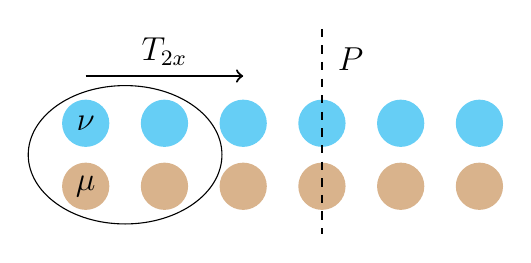
\begin{tikzpicture}
    \foreach \x in {0,...,5}
    \fill[color=brown,opacity=0.6] (\x,0) circle(0.3);
    \foreach \x in {0,...,5}
    \fill[color=cyan,opacity=0.6] (\x,0.8) circle(0.3);
    \draw[rotate=0] (0.5,0.4) ellipse (35pt and 25pt);
    \draw[thick,dashed] (3,2)--(3,-0.6)
    node[pos=0.15,right=2pt] {\large $P$};
    \draw[thick,->] (0,1.4)--(2,1.4)
    node[pos=0.5,above] {\large $T_{2x}$};
    \node at (0,0) {\large $\mu$};
    \node at (0,0.8) {\large $\nu$};
    %\node at (3,-1) {$g\equiv\prod_j\mu^x_j~,\quad h\equiv\prod_j\Big( (\mu^z_j)^2\cdot\nu^x_j\Big)$};
  \end{tikzpicture}
  \caption{The 1D chain system, with local Hilbert space isomorphic to $\mathbb{C}^4\otimes\mathbb{C}^4$. The Hamiltonian is invariant under translational symmetry with two lattice spacing $T_{2x}$, as well as reflection along site center $P$. This system also hosts global $Z_4^g\times Z_4^h$ symmetry generated by $g$ and $h$ defined in Eq.~(\ref{eq:z4_generator_def}), which act projectively on each site, as shown in Eq.~(\ref{eq:z4_proj_rep}).}
  \label{fig:1d_z4z4_spt}
\end{figure}

\subsection{Models and symmetry}
Let us consider a 1D chain system, where the local Hilbert space is isomorphism to $\mathbb{C}^{16}\sim\mathbb{C}^4\otimes\mathbb{C}^4$.
The 16 basis states are labeled as $|\alpha,\beta\rangle$, with $\alpha,\beta=0,1,2,3$.
The Hamiltonian of this system hosts global $Z_4^g\times Z_4^h$ symmetry, which acts projectively on local Hilbert spaces. 

To make the discussion more transparent, it is better to have a concrete model in mind.
{\color{red} It would be better if the Hamiltonian is exact solvable. However, I failed to find such a Hamiltonian.}
Let us consider Hamiltonian in the following form:
\begin{align}
  H=-\sum_j\Big[ &J_1\,\mu^z_{2j-1}(\mu^z_{2j})^\dg\nu^x_{2j}+J_2\,\nu^x_{2j}(\mu_{2j}^z)^\dg\mu_{2j+1}^z+ J_3\,\nu^x_{2j+1} \notag\\
  &+h_1\,\mu^x_{2j}(\nu^z_{2j})^2+h_2\,\nu_{2j}^z\mu^x_{2j+1}\nu^z_{2j+2}+h.c. \Big] +\cdots
  \label{eq:z4z4_reflection_1dspt_ham}
\end{align}
Here $\mu$'s and $\nu$'s are $4\times4$ matrix, which acts as
\begin{align}
  &\mu^z|\alpha,\beta\rangle=\ii^\alpha|\alpha,\beta\rangle~,\quad \mu^x|\alpha,\beta\rangle=|[\alpha+1],\beta\rangle~;\notag\\
  &\nu^z|\alpha,\beta\rangle=\ii^\beta|\alpha,\beta\rangle~,\quad \nu^x|\alpha,\beta\rangle=|\alpha,[\beta+1]\rangle~.
  \label{}
\end{align}
where $[\alpha]\equiv\alpha\!\!\mod 4$.
In particular, we have $\mu^z\mu^x=\ii\mu^x\mu^z$ as well as $\nu^z\nu^x=\ii\nu^x\nu^z$.

Generators of $Z_4^g\times Z_4^h$, labeled as $g$ and $h$, are represented as 
\begin{align}
  g\sim\bigotimes_j\mu^x_j~,\quad h\sim\bigotimes_j (\mu^z_j)^2\cdot\nu^x_j
  \label{eq:z4_generator_def}
\end{align}
in the whole Hilbert space.
It is natural to define the single site action as $W_g(j)\equiv\mu^x_j$, $W_h(j)\equiv(\mu^z_j)^2\nu^z_j$.
Thus, it is straightforward to verify that 
\begin{align}
  &W_g(j)^4=W_h(j)^4=1~,\notag\\
  &W_g(j)W_h(j)=-W_h(j)W_g(j)~.
  \label{eq:z4_proj_rep}
\end{align}
Namely, $Z_4^g\times Z_4^h$ act projectively on the local Hilbert space.

We point out that there are four inequivalent projective representation of $Z_4^g\times Z_4^h$ group, which can be obtained by calculating the second cohomology group: $H^2(Z_4^g\times Z_4^h,U(1))=Z_4$.
These four inequivalent projective representation can be presented as
\begin{align}
  W_g^4=W_h^4=1~,\quad W_gW_h=\ii^\eta\cdot W_hW_g
  \label{}
\end{align}
where $\eta=0,1,2,3$. 
And we use $\eta$ to label the projective representation.
Notice that inequivalent projective representation form an Abelian group, where the group multiplication rule is determined by tensor product of projective representations.
Here, it is easy to verify that the $Z_4$ group multiplication maps to summation of $\eta$'s (\!\!$\mod 4$).
Also, comparing with Eq.~(\ref{eq:z4_proj_rep}), we conclude that the projective representation of $Z_4^g\times Z_4^h$ symmetry supported on the local Hilbert space can be labeled by $\eta_0=2$.

As shown in Fig.~(\ref{fig:1d_z4z4_spt}), Eq.~(\ref{eq:z4z4_reflection_1dspt_ham}) also hosts several lattice symmetry.
Importantly, it is invariant under site-center reflection $P$ as well as two lattice-spacing translation $T_{2x}$, which read as
\begin{align}
  &P:\mu_{j}\rightarrow\mu_{-j}~,\quad\nu_{j}\rightarrow\nu_{-j}~;\notag\\
  &T_{2x}:\mu_j\rightarrow\mu_{j+2}~,\quad\nu_j\rightarrow\nu_{j+2}~.
  \label{}
\end{align}
where we ignore subscripts of $\mu_j(\nu_j)$ for brevity.
We point out that $\cdots$ in Eq.~(\ref{eq:z4z4_reflection_1dspt_ham}) represents other terms respecting above global symmetries.

\begin{figure}[h]
  \centering
  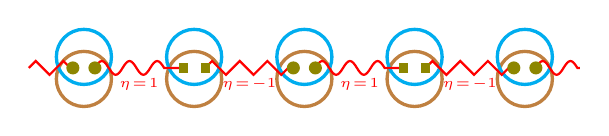
\begin{tikzpicture}[scale=1.4]
    \foreach \x in {0,...,4}
    \draw[color=brown,very thick] (\x,-0.1) circle(0.25);
    \foreach \x in {0,...,4}
    \draw[draw=cyan,very thick] (\x,0.1) circle(0.25);
    \draw[thick,color=red,snake=zigzag] (-0.5,0) -- (-0.1,0) node[circle,fill,color=olive,scale=0.5] {};
    \draw[thick,color=red,snake=coil,segment aspect=0] (0.1,0) node[circle,fill,color=olive,scale=0.5]{}  --(0.9,0) node[fill,color=olive,scale=0.5]{} node[pos=0.5,below]{\tiny$\eta\!=\!1$};
    \draw[thick,color=red,snake=coil,segment aspect=0] (2.1,0) node[circle,fill,color=olive,scale=0.5]{}  --(2.9,0) node[fill,color=olive,scale=0.5]{} node[pos=0.5,below]{\tiny$\eta\!=\!1$};
    \draw[thick,color=red,snake=zigzag] (1.1,0) node[fill,color=olive,scale=0.5]{} --(1.9,0) node[circle,fill,color=olive,scale=0.5]{} node[pos=0.5,below]{\tiny$\eta\!=\!-1$};
    \draw[thick,color=red,snake=zigzag] (3.1,0) node[fill,color=olive,scale=0.5]{} --(3.9,0) node[circle,fill,color=olive,scale=0.5]{} node[pos=0.5,below]{\tiny$\eta\!=\!-1$};
    \draw[thick,color=red,snake=coil,segment aspect=0] (4.1,0) node[circle,fill,color=olive,scale=0.5] {} -- (4.5,0);
    %\node at (0,0) {\large $\mu$};
    %\node at (0,0.8) {\large $\nu$};
  \end{tikzpicture}
  \caption{A natural candidate for symmetric phases of system defined in Eq.~(\ref{eq:z4z4_reflection_1dspt_ham}). The construction is similar as the famous AKLT state[].}
  \label{fig:1d_z4z4_spt}
\end{figure}

Now, let us discuss possible phases for Eq.~(\ref{eq:z4z4_reflection_1dspt_ham}).
In particular, we will focus on possible gapped phases with no spontaneously symmetry breaking.
A natural candidate for symmetric phases is shown in Fig.~(\ref{fig:1d_z4z4_spt}).
The construction is similar as the famous AKLT phase[]: an $\eta=2$ state is decomposed to two $\eta=1(-1)$ states, and the $\eta=1$ state from the left/right site pairs with the $\eta=-1$ state from the right/left site.
Consequently, if one puts the system on an open boundary, there will be an unpaired $\eta=1$ or $\eta=-1$ zero mode at each boundary.

%It is natural to ask, is it possible to obtain other symmetric phases, such as phases without nontrivial edge modes? 
In integer spin chain with $SO(3)$ symmetry, depending on the interaction, one can either get Haldane phase[] with spin-1/2 on the boundary, or obtain symmetric phase[] without nontrivial edge modes.
However, for the system discussed above, we will argue that all possible gapped symmetric phases must be nontrivial SPT phases, in the sense that they host degenerate zero modes on boundaries. 

\subsection{Entanglement based argument}
The following argument is based on entanglement properties.
Given a quantum many-body wavefunction $|\psi\rangle$ on a 1D chains, one can ``cut'' the system to two halves along bond $(j,j+1)$ and do Schmit decomposition as
\begin{align}
  |\psi\rangle=\sum_i\lambda_i|\phi^L_i\rangle\otimes|\phi^R_i\rangle
  \label{}
\end{align}
where $|\lambda_1|\le|\lambda_2|\le\cdots$. 
$|\phi^{L/R}(i)\rangle$ are named as left/right entanglement states (respect to bond $(j,j+1)$).
It is well known that if $|\psi\rangle$ describes gapped symmetric ground state, the entanglement spectrum, defined as $\{-\ln|\lambda_i|^2\ |\ i=1,2,\cdots\}$, is also gapped[] in the thermodynamic limit.
Furthermore, entanglement states transform projectively under the on-site symmetry group.
Namely, for $g\in SG_{onsite}$, 
\begin{align}
  U_{g}^{L/R}|\phi^{L/R}_i\rangle=\sum_k (W_{g}^{L/R})_{ik}|\phi^{L/R}_k\rangle
  \label{}
\end{align}
where $U_{g}^{L/R}$ is the physical symmetry action which acts on left/right system of bond $(j,j+1)$.
And $W_g$ in general form some projective representation of $SG$.
In particular, for $Z_4^g\times Z_4^h$ group, we have
\begin{align}
  &\sum_{k}(W_{g}^{L/R}\cdot W_h^{L/R})_{ik}|\phi^{L/R}_k\rangle\notag\\
  =&\exp[\ii\frac{\pi}{2}\cdot\eta^{L/R}_{j+1/2}]\sum_{k} (W_h^{L/R}\cdot W_g^{L/R})_{ik}|\phi^{L/R}_k\rangle
  \label{}
\end{align}
where $\eta^{L/R}_{j+1/2}=\{0,1,2,3\}$ can be used to label the projective representation of entanglement states at bond $(j,j+1)$.
%and that of the right-half system as $\eta^R_{j+1/2}$.
%By definition, we have $\eta^L_{j+1/2}=-\eta^R_{j+1/2}$, where ``='' is defined up to 4.

Now, we are ready to argue the possible symmetric phases for this system.
{\color{red} More derivation (based on MPS) about symmetry constraint on $\eta$?}
First, due to $Z_4^g\times Z_4^h$ global symmetry, we conclude
\begin{align}
  \eta^R_{j+1/2}+\eta^L_{j+1/2}=0~,\quad \eta^R_{j-1/2}+\eta^L_{j+1/2}=\eta_0
  \label{}
\end{align}
where ``='' is defined up to 4, and $\eta_0=2$ labels site projective representation.
Second, from reflection symmetry along site $j$, we have 
\begin{align}
  \eta^R_{j-1/2}=\eta^L_{j+1/2}
  \label{}
\end{align}
We also impose translational symmetry, which requires
\begin{align}
  \eta^{L/R}_{j-1/2}=\eta^{L/R}_{j+3/2}
  \label{}
\end{align}
By solving above equations, we then get solution $\eta^{L/R}_{2j-1/2}=\eta^{R/L}_{2j+1/2}=\pm1$.
The nonzero $\eta$ also indicates edge modes transform projectively under $Z_4^g\times Z_4^h$ symmetry, and the symmetric phases obtained are always nontrivial SPT phases.

Furthermore, we can easily see that it is essential to require $\eta_0=2$ on every site.
If $\eta_0=1(3)$, we get never find an integer solution for $\eta^{L/R}$, which exclude the possibility to have gapped symmetric phases.
Indeed, in this case, in each unit cell, there is nontrivial projective representation with $\eta=2$, which indicates LSM ``anomaly'', and exclude gapped symmetric phases.
On the other hand, if $\eta_0=0$, as one expects, there is a trivial solution with $\eta^{L/R}=0$, which gives trivial gapped symmetric phase.

\subsection{SPT phases from domain wall condensation}
In the following, we will argue the possible symmetric phases from domain wall point of view.
The domain wall condensation picture would provide more insights on possible SPT phases, and it would also give us more hints to construct models realizing SPT phases.

Now, let us perform the $Z_4$ version of Kramers-Wannier duality. We define
\begin{align}
  \tau^x_{j+1/2}=(\mu^z_j)^\dg\mu^z_{j+1}~,\quad \tau^z_{j+1/2}\equiv\prod_{k\le j}\mu^x_j
  \label{eq:z4_dw_duality}
\end{align}
where $\tau^z_{j+1/2}\tau^x_{j+1/2}=\ii \tau^x_{j+1/2}\tau^z_{j+1/2}$.
Here, $\tau^x_{j+1/2}$ measures $g$ domain wall at bond $(j,j+1)$, while $\tau^z_{j+1/2}$ is $g$ domain wall creation operator.

%We point out that in a periodic chain, a unit $g$ domain wall is not local object, which should always appear with its anti-particle.
%Thus, to capture global aspects and identify phases of original model, it is better to introduce a $\widetilde{Z_4}$ gauge field, and treat $g$ domain walls as $\widetilde{Z_4}$ gauge charges.
%This would lead to two consequence.
%First, $\widetilde{Z_4}$ (spacetime) flux carries $Z_4^g$ symmetry charge, and gapped phase of $g$ domain wall would lead to $g$ symmetry breaking, due to $\widetilde{Z_4}$ flux condensation.
%Second, $g$ domain wall has an additional $\widetilde{Z_4}$ symmetry, 
%can carry nontrivial projective representation of other symmetry group.

Equipped with the mapping defined in Eq.~(\ref{eq:z4_dw_duality}), we are able to work out the symmetry action on $g$ domain wall:
\begin{align}
  &h:\tau^z_{j+1/2}\rightarrow (-)^j\tau^z_{j+1/2}\notag\\
  &P:\tau^z_{j+1/2}\rightarrow (\tau^z_{-j-1/2})^\dg\notag\\
  &T_{2x}:\tau^z_{j+1/2}\rightarrow \tau^z_{j+2+1/2}
  \label{eq:z4_dw_sym_action}
\end{align}
Besides, there is an additional $\widetilde{Z_4^g}$ domain wall ``conservation'' symmetry, which is generated by $\widetilde{g}=\prod_j\tau^x_{j+1/2}$, and acts as
\begin{align}
  \widetilde{g}: \tau^z_{j+1/2}\rightarrow-\ii\tau^z_{j+1/2}
  \label{}
\end{align}

Now, let us consider possible phases obtained from domain wall variables.
If domain wall is disordered, meaning $\langle\tau^z\rangle=0$, $Z_4^g$ symmetry would be broken.
Thus, we would like to focus on the condensation phase of domain wall.
We point out that naive condensation pattern of domain walls would always break global symmetries.

To see this, let us calculate commutation relation between $h$ and $P$ when acting on domain walls:
\begin{align}
  hP\circ\tau^z=-Ph\circ\tau^z(\equiv\widetilde{g}^2 Ph\circ\tau^z)
  \label{eq:dw_z4P_proj_rep}
\end{align}
This anti-commutation relation indicates that the representation of symmetry group on $\tau^z$ must be non-Abelian.

We point out that, since domain walls are non-local objects, in general, $\tau^z$ forms a projective representation of $SG$ with $\widetilde{Z_4^g}$ coefficient.
In other words, $\tau^z$ form a linear representation of $PSG$[Wen], which is defined as an $SG$ extension by $\widetilde{Z_4^g}$, where $SG$ is the global symmetry group including both onsite and space symmetry.
In the current settings, all possible $PSG$ is classified by second group cohomology with coefficient $\widetilde{Z_4^g}$: $H^2\left[ SG,\left(\widetilde{Z_4^g}\right)_P \right]$.
Here, the subscript $P$ denotes the nontrivial action of reflection on $\widetilde{Z_4^g}$:
\begin{align}
  P\cdot\widetilde{g}\cdot P^{-1}\circ\tau^z=\widetilde{g}^{-1}\circ\tau^z
  \label{eq:dw_Pigg_action}
\end{align}
If $PSG$ corresponds to a nontrivial element in $H^2$, condensing domain walls would always leads to spontaneous symmetry breaking.
{\color{red} Illustrate more on the effect of condensing domain walls with nontrivial PSG?}

Naively, Eq.~(\ref{eq:dw_z4P_proj_rep}) seems indicate the nontrivial group extension.
However, by redefining $h\rightarrow \widetilde{g}h$ and use Eq.~(\ref{eq:dw_Pigg_action}), it turns out that $P$ and $h$ commute when acting on $\tau^z$.
In other words, the group extension here is trivial.
Thus, it is possible to have symmetric phases by condensing domain walls .

However, due to symmetry action defined in Eq.~(\ref{eq:z4_dw_sym_action}), it turns out that any condensation pattern of $\tau^z$ would lead to breaking of either $Z_4^h$ symmetry or $P$ symmetry.
%Since domain walls are non-local variables, one needs to be more careful about the effect of domain wall condensation.
%It is actually better to treat $\widetilde{g}$ as ``gauge symmetry'', and local observables should always carry trivial gauge charge under $\widetilde{g}$, which include terms as $(\tau^z)^\dg\tau^z$, $\tau^z\tau^z\tau^z\tau^z$, etc.
%Condensation of $\tau^z$ leads to non-zero expectation value of some gauge-neutral terms.
%Notice that the global symmetry representation of those terms is obtained by tensor product of the representation of single $\tau^z$.
%Since $\tau^z$ carries non-Abelian representation under global symmetry group, as shown in Eq.~(\ref{eq:dw_z4P_proj_rep}), any gauge neutral term made of $\tau^z$ must also carry nontrivial symmetry charge, which leads to symmetry breaking phases.
Let us give examples to illustrate the above argument.
For example, let us consider condensation pattern to be $\langle\tau^z_{j+1/2}\rangle\neq0$ and is independent of $j$.
It will preserve $P$ symmetry, but break $Z_4^h$ to $Z_2$ subgroup. 
To see this, we consider local operator $(\tau^z_{2j-1/2})^\dg\tau^z_{2j+1/2}$. 
Under $Z_4^h$ transformation, this operator obtains minus sign, thus carry two $Z_4^h$ charge.
Then, with $\langle\tau^z_{j+1/2}\rangle\neq0$, this operator would pick nonzero expectation value and break $Z_4^h$ to $Z_2$.
On the other hand, we may also condense $\tau^z_{2j+1/2}$ but leave $\tau^z_{2j-1/2}$ gapped.
In this case, $Z_4^h$ is preserved, since $\tau^z_{2j+1/2}$ is invariant under $Z_4^h$ (up to some $\widetilde{Z_4^g}$ transformation).
However, this condensation pattern would break $P$ symmetry.

To obtain a fully symmetric phase, the key step is to condense the bound state of $g$ domain wall and $h$-charge $\tau^z\nu^z$ or $\tau^z(\nu^z)^\dg$.
In particular, we choose the condensation pattern as $|\langle\tau^z_{2j-1/2}(\mu^z_{2j})^\dg\rangle|=|\langle\mu^z_{2j}\tau^z_{2j+1/2}\rangle|=\alpha\neq0$.
It is straightforward to check that under this condensation pattern, all gauge neutral objects with non-zero expectation value are invariant under global symmetry action.
Thus, we obtain a symmetric gapped phase.
Furthermore, from decorated domain wall point of view[Chen,Lu,Vishwanath], condensation of bound states of domain walls and symmetry charges leads to SPT phases.

The above condensation pattern also gives us hint to construct Hamiltonian realizing the symmetric phases.
\ldots

Now, let us summarize the argument about domain wall condensation, which would be helpful for us to generalize similar argument to high dimension.
\begin{enumerate}
  \item Gapped domain wall always leads to $Z_4^g$ symmetry breaking phases.  
    From gauge theory perspective, it is due to the fact gauge (spacetime) flux carries $Z_4^g$ charge. 
    Gapped gauge charge leads to condensation of flux in 1+1D, which spontaneously breaks $Z_4^g$ symmetry.  
  \item $PSG$ for domain walls~(or $\widetilde{Z_4^g}$ gauge charges) are trivial extension of $SG$ by $\widetilde{Z_4^g}$.
    However, condensing ``bare'' domain walls $\tau^z$ always gives spontaneous symmetry breaking phases.
  \item By condensing some bound state of domain wall $\tau^z$ and some global symmetry charge, we are able to get fully symmetric phases.
    As a result, the phase we obtained is SPT state with nontrivial edge zero modes.
\end{enumerate}
From domain wall condensation picture, one can also obtain the possible phases for other $\eta_0$.
For example, when $\eta_0=1$, one is able to show $PSG$ now is a nontrivial extension of $SG$ by $\widetilde{Z_4^g}$.
Thus, condensing domain walls would always give symmetry breaking phases.
On the other hand, for the case with $\eta_0=0$, one is able to condensing ``bare'' domain wall $\tau^z$ without breaking any symmetry, which gives the trivial SPT phase.

\subsection{Construction from spectral sequence}
{\color{red} Calculate group cohomology $H^2(Z_4^g\times Z_4^h\times Z_2^P,U_P(1))$ to show this SPT phase is not included in the conventional SPT classification.}


\section{General framework}\label{sec:general_framework}
The 1D example presented in the last section can be generalized to higher dimensions and to other symmetry groups.

We focus on boson/spin systems in this paper.
One of the main goals in condensed matter physics is to study phase diagrams for a given Hamiltonian with some tunable parameters.
To figure out the phase diagram of a given model, the first step is to classify possible phases for this model, which is also much easier to solve.
We concentrate on a subclass of possible phases: symmetric SRE phases, namely, SPT phases.

\subsection{The global symmetry group and local Hilbert spaces}
To classify possible (SPT) phases, we do not have to know all details about microscopic Hamiltonians.
The crucial information is the global symmetry group of the model, labeled as $SG$, which includes both spatial and onsite symmetry actions.
Naively, one may think $SG$ contains enough input data for the purpose of classification of SPT phases.
It is indeed true if $SG$ is onsite symmetry group. 
In this case, various mathematical tools are proposed to classify SPT phases, including group cohomology\cite{ChenGuLiuWen2013}, cobordism theory[\ldots], generalized cohomological theory[\ldots], \ldots

When $SG$ contains lattice symmetries, the classification problem becomes more tricky.
On the one hand, researchers argued that one should treat spatial symmetries and onsite symmetries on the same footing, and the classification of SPT phases is given by group cohomology $H^{d+1}[SG,U(1)]$, with time reversal and orientation reversing lattice symmetries act nontrivially on $U(1)$ coefficient\cite{JiangRan2017,ThorngrenElse2018gauging}.\footnote{There are phases beyond group cohomological classification[Hermele\ldots]. We will not focus on those phases in this paper.}
On the other hand, a more physical way to understand SPT phases protected by both spatial and onsite symmetries is the dimension reduction picture[Hermele\ldots], which provides construction of SPT phases by decorating high-symmetry points, lines and planes with lower dimensional onsite symmetry SPT phases.
It has been shown that this ``real-space'' construction is one-to-one correspondence to classes in $H^{d+1}[SG,U(1)]$[Yang].

It is worth mentioning that when deriving the above classification result, one actually takes a hidden assumption: local Hilbert spaces are linear representations of the corresponding little groups.
However, local Hilbert spaces can also support nontrivial projective representations.
In the absence of lattice symmetry, this fact does not change the classification. {\color{red} How to argue this?}
Yet when we include lattice symmetry, projective representations play an important role in the classification result.
To see this, let us consider an example of translational symmetric spin chains.
There are two kinds of translational symmetric spin chains, which are integer spin chains and half-integer spin chains.
They share the same global symmetry group: $SO(3)\times Z$. 
Yet possible phases of these two systems are completely different.
For integer spin chains, classification of SPT phases equals $Z_2$, corresponding to the trivial SPT phase and the Haldane phase.
For half-integer spin chains, one is never able to construct a gapped symmetric phase, according to the original LSM theorem.

From the above example, we learned that for systems with the same global symmetry group but different local Hilbert spaces, the possible SPT phases are in general different.
Thus, to study possible SPT phases for a given system, one at least needs both global symmetry group as well as structures of local Hilbert spaces.
So, the first step is to classify local Hilbert spaces according to their projective representations.
{\color{red} $SG$-complex, cell decomposition, projective rep data $E^1_{0,r}$}

%Here, we are particularly interested in systems with following constraints on quantum phases:
%\begin{enumerate}
%  \item These systems are able to support symmetric SRE phases.
%  \item Yet it is impossible to have trivial symmetric phases. 
%    Namely, all possible symmetric SRE phases on these systems are nontrivial SPT phases.
%\end{enumerate}
%We call such systems SPT-LSM systems. 
%It is natural to ask the following questions:
%\begin{enumerate}
%  \item For a bosonic system with a given symmetry group and local Hilbert spaces, are we able to tell if it is an SPT-LSM system?
%    If the answer is yes, what are allowed SPT phases?
%  \item Is there any guiding principle to find an SPT-LSM system to realize some particular SPT phase? 
%\end{enumerate}
%In this section, we will emphasize the first question.
%We develop a general framework to tell whether the system is an SPT-LSM system and also to determine constraints on possible SPT phases.

\subsection{First page result}

\subsection{High page result}

{\color{red} Mathematical structure to describe this classification?}


\section{Examples for SPT-LSM systems in higher dimension}\label{sec:higher_dim_spt_lsm}
Based on techniques developed in Section~\ref{sec:general_framework}, given global symmetry $SG$ and local Hilbert spaces, one is able to figure out constraints on possible SPT phases.
In this section, we are interested in the ``inverse problem'': 
given the constraint on SPT phases, is there way to figure out the corresponding SPT-LSM systems which realize the constraint?
Here, we propose a method to find such systems, which is based on the idea to obtain SPT phases by condensation of gauge charges in a symmetric gauge theory.
Details of this condensation mechanism can be found in Appendix~\ref{app:SPT_condensation}.
In this section, we focus on strong SPT phases, namely, SPT phases protected by onsite symmetry alone.
For examples on high-order/weak SPT phases, we refer to Appendix~\ref{app:weak_spt_lsm}.

\subsection{SPT phase protected by $Z_2^s\times Z_2^\TT$ in 2+1D}\label{subsec:z2hT_spt_2+1}
Let us consider SPT phases protected by onsite symmetry $Z_2^s\times Z_2^\TT=\{1,s\}\times\{1,\TT\}$.
According to cohomology classification, we have $H^3[Z_2^s\times Z_2^\TT,U(1)]=Z_2^2$, where one $Z_2$ root phase, labeled as $\nu_s$, is the famous Levin-Gu SPT phase protected by $Z_2^s$ symmetry only\cite{LevinGu2012}, while the other $Z_2$ root phase, labeled as $\nu_{s\TT}$, is the SPT phase due to interplay between $Z_2^s$ and $Z_2^\TT$. 
This phase can be understood from decorated domain wall picture: domain walls of $Z_2^s$ are decorated by $Z_2^\TT$ Haldane chains\cite{ChenLuVishwanath2014}.

We will find systems with the SPT phase $\nu_{s\TT}$ as the ``minimal required'' SRE phase. 
We mention that one example based on magnetic translation group is presented in Ref.~\onlinecite{YangJiangVishwanathRan2018}.
Here, we give a new SPT-LSM system by replacing magnetic translation with ``magnetic inversion''.
This SPT-LSM system has, in addition to the $Z_2^s\times Z_2^\TT$ onsite symmetries, a spatial inversion symmetry $\widetilde{\II}$ such that $\widetilde{\II}^2=s$. The SPT-LSM condition is that there is one Kramers doublet at the inversion center.

This SPT-LSM theorem can be understood from anyon condensation in a symmetric gauge theory. This "parent" phase is realized in a lattice system with spatial inversion symmetry $\II$ satisfying $\II^2=1$ and an onsite time-reversal symmetry $\TT$, such that there is a Kramers doublet at the inversion center. We present the argument in several steps:
\begin{enumerate}
  \item The first step is to identify a symmetric gauge theory, whose gauge charge condensation would result in the desired SPT phase.

    For the case considered here, we start from a $Z_2$ toric code topological order with global symmetry $Z_2^s\times Z_2^\TT$, where the gauge fluxon $m$ transforms as a Kramers doublet under $Z_2^\TT$ and the gauge charge $e$ transforms trivially under the onsite global symmetry:
    \begin{align}
      &\TT^2\circ m=-m~,\quad s^2\circ m=s~;\notag\\
      &\TT^2\circ e=s^2\circ e=e~.
      \label{eq:z2z2t_set_before_cond}
    \end{align}
    The SPT phase $\nu_{s\TT}$ can be obtained by condensing bound state of $e$ and a $Z_2^s$ charge excitation $\RR_s$\cite{JiangRan2017}.
    Details of condensation mechanism are presented in Appendix~\ref{subapp:anyon_condensation}.
  \item As we have mentioned, the symmetric gauge theory must be realized in a lattice with the ``parent" LSM theorem. For the symmetric gauge theory to ``resolve" the LSM constraint, we let the gauge charge $e$ transform projectively under inversion symmetry:
    \begin{align}
      \II^2\circ e=-e~;\notag\\
      \label{}
    \end{align}
    The onsite symmetry fractionalization pattern is still given by Eq.~(\ref{eq:z2z2t_set_before_cond}).
    Due to nontrivial symmetry action on both $e$ and $m$, condensing either quasiparticle would lead to symmetry breaking phase, as required by the LSM theorem.
  \item The last step is to modify symmetry group, so that symmetry charges transform oppositely from gauge charges under lattice symmetry.
    Thus, bound state of gauge charges and symmetry charges transform trivially under the modified symmetry group.

    In this LSM system, by condensing bound state of $e$ and $\RR_s$, we would get the desired SPT, but break inversion symmetry $\II$ at the mean time.
    To avoid symmetry breaking, we replace $\II$ with ``magnetic inversion'' $\widetilde{\II}$, where $\widetilde{\II}^2=s$. 
    For $\widetilde{II}$ action, we have
    \begin{align}
      \widetilde{\II}^2\circ R_s=-R_s~,\quad \widetilde{\II}^2\circ e=-e
      \label{}
    \end{align}
    And condensing bound state of $e$ and $\RR_s$, we obtain the desired SPT without breaking any lattice symmetry.
\end{enumerate}

Let us also comment on the meaning of ``minimal required'' SPT phase. 
We point out that SPT phases obtained in this system is not unique.
In this example, notice that symmetry action on the $Z_2$ gauge theory is not uniquely determined.
For example, we could have $s^2\circ m=- m$, and condensing bound state in this case would lead to phase $\nu_s\nu_{s\TT}$, shown in Appendix~\ref{subapp:anyon_condensation}.
Yet for any SPT phases realized in this system, $Z_2^s$ defects are always Kramers doublets.

However, the above anyon-condensation argument does not exclude the possibility of trivial SPT phase in this system. Below we provide an entanglement-based argument to prove that any gapped symmetric ground state must be a SPT phase protected by $Z_2^s\times Z_2^\TT$ symmetry. 

Without loss of generality, we consider a square lattice model, where Ising charges (neutral under time reversal $\TT$) live on each lattice site ${\bf r}=(x,y)\in\mathbb{Z}^2$. Besides, there is a Ising-neutral spin-$1/2$, which is a projective representation of time reversal symmetry $\TT$, living on each plaquette center $(x+\frac12,y+\frac12)$. The magnetic inversion symmetry $\tilde\II$ is implemented as
\begin{eqnarray}
  &\tilde\II\equiv\big[\prod_{\bf r}(s_{\bf r})^y\big]\cdot\II,\\
  &(x,y)\overset{\II}\longrightarrow(1-x,1-y).\notag
\end{eqnarray}
where we have chosen the inversion center to be each plaquette center. It is straightforward to check that
$\tilde\II^2=\prod_{\bf r}s_{\bf r}=s$ is indeed satisfied, where $s_{\bf r}$ denotes $Z_2$ spin rotation on each site ${\bf r}$. 

One can always embed the $Z_2$ Ising symmetry $s$ in a $U(1)$ group, for example by choosing 
\begin{eqnarray}
  s=e^{i\pi\hat Q},~~~s^2=e^{2\pi i\hat Q}=1,\\
  \notag U(1)\equiv\{e^{i\phi\hat Q}|0\leq\phi<2\pi\}.
\end{eqnarray}
The magnetic inversion symmetry $\tilde\II$ implements the following constraint on the $U(1)$ vector potential
\begin{eqnarray}
  \vec A(1-x,1-y)=-\vec A(x,y)+(0,\pi).
\end{eqnarray}
which has the following solution in the Landau gauge
\begin{eqnarray}
  \vec A(x,y)=(0,\pi x)
\end{eqnarray}
This implies the presence of a $\pi$ flux (i.e. an Ising symmetry flux) in each plaquette, in addition to the spin-$1/2$ at the plaquette center. Notice that in addition to the magnetic inversion symmetry $\tilde\II$, the system also preserves magnetic translation symmetries, for example 
\begin{eqnarray}
  \tilde T_x=\big[\prod_{\bf r}(s_{\bf r})^y\big]\cdot T_x,~~~\tilde T_y=T_y.
\end{eqnarray}
When put on a cylinder with infinite length $L_x\longrightarrow+\infty$ and an \emph{odd} circumference $L_y=$~odd, the boundary condition along $\hat y$ direction oscillates between periodic and anti-periodic boundary conditions between different columns $x=$~even and $x=$~odd. Therefore by analyzing its entanglement spectrum at two different cuts $\bar x=\epsilon$ and $\bar x=1-\epsilon$ related by inversion symmetry $\tilde\II$, we can use the same argument in Ref.\cite{Wu2017,Lu2017b,YangJiangVishwanathRan2018}, we can show a gapped symmetric ground state cannot be a trivial product state, but instead has to be a SPT phases constructed by decorating $Z_2^s$ domain wall with 1d $Z_2^\TT$ SPT phase. 

{\color{red}  Spectral sequence calculation for this system?}

We now briefly describes a model that realizes such a SPT-LSM system.
{\color{red} Models realize this SPT phase?}

BLG-Ising model, where inversion is chosen to be the hexagon center with a spin-$1/2$? 


\subsection{SPT phase protected by $U_s(1)\times Z_2^\TT$ in 3+1D}
Following the procedure summarized in last part, here we will propose systems enforcing bosonic SPT phase in 3+1D with onsite symmetry group $U_s(1)\times Z_2^\TT$.
Here $U_s(1)$ can be viewed as spin rotation symmetry along $z$-axis.
Cohomological group calculation would give $Z_2^3$ classification\cite{ChenLuVishwanath2014}, while there is another $Z_2$ class beyond cohomology\cite{VishwanathSenthil2013,Kapustin2014}.
Properties of cohomological SPT phases, as well as approaches to obtain these phases from monopole condensation are discussed in Appendix~\ref{subapp:monopole_cond}.

In this part, we focus on a particular $Z_2$ root state, which can be detected by statistical Witten effect\cite{Witten1979,MetlitskiKaneMatthew2013}: the external monopole of $U_s(1)$ is a fermionic excitation.

Following the last part, we first identify a possible route to obtain this SPT phase from condensing quasiparticles of a symmetric gauge theory
A possible way is to start from a compact $U_g(1)$ quantum spin liquid~(QSL). 
Excitations of the $U_g(1)$ QSL includes gauge charges, monopoles as well as photons.
For the purpose of this part, we can safely ignore photons, but focus on symmetry properties of gauge charges and monopoles.
We mention that monopoles can be viewed as gauge charges of a dual $\widetilde{U_g}(1)$ gauge field. 
And we focus on phase obtained from monopole condensation here.

We consider the case where gauge charge, labeled as $b_g$, carries half-charge of $U_s(1)$, while monopole $M_g$ carries trivial quantum number. 
We claim that condensing bound state of monopole $M_g$ and a unit $U_s(1)$ charge would lead to the desired SPT phase with fermionic external monopole of $U_s(1)$.
Notice that monopole $M_g$ of $U_g(1)$ gauge field and external monopole of $U_s(1)$ are two different objects, and should not be confused with each other. 
The detailed argument for this condensation mechanism is presented in Appendix~\ref{subsubapp:fermionic_monopole_SPT}.

Now, let us be more precise about symmetry properties of this QSL.
Under global symmetry $U_s(1)\times Z_2^\TT$, we require the transformation rule as
\begin{align}
  U_s(\theta)&: b_{g}\rightarrow \ee^{\ii\sigma^z\frac{\theta}{2}}\cdot b_{g}~,\quad M_g\rightarrow M_g~;\notag\\
  \TT&: b_{g}\rightarrow \sigma^x \cdot b_{g}~,\quad M_g\rightarrow M_g^\dg~,\quad \ii\rightarrow-\ii~.
  \label{eq:U1_QSL_charge_monopole_sym_action}
\end{align}
where $b_g=(b_{g\uparrow},b_{g\downarrow})^\mathrm{t}$ is a two component operator with spin index.
We point out an important distinction between onsite unitary and anti-unitary symmetries.
Under onsite unitary symmetry action, both $b_g$ and $M_g$ should either remain in the same topological sector or transform to antiparticles.
However, for under onsite anti-unitary action, if gauge charges transform to their antiparticles, monopoles must remain in the same sector, and vice versa.

It is possible to realize this $U_g(1)$ QSL by a local spin-1/2 model with symmetry action on spin operator $\vec{S}$ as
\begin{align}
  U_s(\theta)&: S^+\rightarrow \ee^{-\ii\theta} S^+,\quad S^z\rightarrow S^z~,\notag\\
  \TT&: S^{\pm}\rightarrow S^{\mp},\quad S^z\rightarrow-S^z,\quad \ii\rightarrow-\ii~.
  \label{eq:3+1_spin_sym}
\end{align}
Namely, symmetry operators are
\begin{align}
  U_s(\theta)\sim \exp\left( -\ii\theta S^z \right)~,\quad \TT\sim S^x\KK
  \label{}
\end{align}

In this system, $U_g(1)$ gauge charge $b_g$ can be constructed by partons of spin operator
\begin{align}
  \vec{S}\sim\frac{1}{2}b_g^\dg\cdot \vec{\sigma}\cdot b_g
  \label{eq:parton_construction}
\end{align}
The desired SPT phase is obtained by condensing the bound state of $M_g$ and $S^+$.

Having identified the symmetric gauge theory, the next step to figure out a 3+1D LSM system, which is able to support this $U_g(1)$ gauge theory with the same onsite symmetry action defined in Eq.~(\ref{eq:U1_QSL_charge_monopole_sym_action}).
For this purpose, we consider a cubic lattice, with single spin-1/2 living on each lattice site.
Global onsite symmetry action is defined in Eq.~(\ref{eq:3+1_spin_sym}).
Translational symmetries $T_{x,y,z}$ are imposed, and there is one spin-1/2 per unit cell.
We also require translation act nontrivially on spin operator as
\begin{align}
  T_i:S^{\pm}(j)\rightarrow S^{\mp}(j+\hat{e}_i)~,\quad -S^z(j)\rightarrow S^z(j+\hat{e}_i)~.
  \label{eq:transl_action_spin_1/2}
\end{align}
where $i=x,y,z$ and $\hat{e}_i$ denotes the lattice constant along $i$ direction.

This system has LSM anomaly, which disallows symmetric SRE phase. 
{\color{red} We should argue this system has LSM anomaly, e.g. by constructing 4D SPT bulk?}
Yet we are able to construct $U_g(1)$ QSL phase with the same onsite symmetry properties defined in Eq.~(\ref{eq:U1_QSL_charge_monopole_sym_action}) on this system by parton construction Eq.~(\ref{eq:parton_construction}).
A single spin-1/2 per unit cell indicates nontrivial background gauge charge distribution in the context of $U_g(1)$ QSL: there are $2k+1$ positive gauge charges living on even lattice site, and $-2k-1$ gauge charges living on odd lattice site.
Here, for lattice site $j=(j_x,j_y,j_z)$, even/odd lattice site means $j_x+j_y+j_z$ is an even/odd number.
{\color{red} How to justify the background gauge charge distribution picture?}

Notice that translation operator $T_i$ act similarly as particle-hole symmetry on $b_g$: $b_g(j)\rightarrow b_g^\dg(j+\hat{e}_i)$ (up to some phase factor) under translations.
This is consistent with translation action on spin operators in Eq.~(\ref{eq:transl_action_spin_1/2}) and also consistent with gauge charge distributions discussed above.
%In particular, we are able to choose translational action as
%\begin{align}
%  T_\alpha: b_g(j)\rightarrow b_g^\dg(j+\hat{\alpha})~,\quad \alpha=x,y,z
%  \label{}
%\end{align}

Due to the background gauge charge distribution, magnetic monopole $M_g$ would acquire nontrivial Berry phase when hopping around a closed loop.
A specific hopping ansatz for $M_g$ is given in Ref.~\onlinecite{MotrunichSenthil2005}, which we review on Appendix~\ref{app:mf_ansatz_monopole}.
According to this mean field ansatz, we are able to extract translation action on $M_g$ as
\begin{align}
  &T_x: M_g(j)\rightarrow M_g^\dg(j+\hat{x})~, \notag\\
  &T_y: M_g(j)\rightarrow M_g^\dg(j+\hat{y})~, \notag\\
  &T_z: M_g(j)\rightarrow \ii^{(x+y)^2+2x}M_g^\dg(j+\hat{z})~.
  \label{eq:monopole_translation_action}
\end{align}
%Notice that translation action on gauge charges and monopoles is similar as onsite unitary symmetry action, in the sense that they both map both $b_g$ and $M_g$ to their anti-particles.
As shown in Ref.~\onlinecite{MotrunichSenthil2005}, condensation of monopole breaks translational symmetry, and the pattern of VBS order parameter depends on details of condensation.

As discussed in detail on Appendix~\ref{subsubapp:fermionic_monopole_SPT}, condensation of the bound state of $M_g$ and $S^+$ leads to the SPT phase with fermionic external $U_s(1)$ monopole.
Yet this condensation breaks translational symmetry according to Eq.~(\ref{eq:transl_action_spin_1/2}) and Eq.~(\ref{eq:monopole_translation_action}).
To avoid symmetry breaking, we should modify definition of translations in Eq.~(\ref{eq:transl_action_spin_1/2}).
Equivalently, we choose a particular hopping ansatz for $S^+$, which is complex conjugate of ansatz for $M_g$.
Thus, the bound state will hop in a zero flux background.
By condensing the bound state at $\Gamma$ point, we would get a symmetric SRE phase, with the desired SPT index.
Let us identify the modified translation symmetries for this $S^+$ hopping ansatz.
Since background flux for $S^+$ would be opposite to flux for $M_g$, translation symmetry action on spin operators becomes
\begin{align}
  &T_x: S^+(j)\rightarrow S^-(j+\hat{x})~,\quad S^z(j)\rightarrow -S^z(j+\hat{x})~; \notag\\
  &T_y: S^+(j)\rightarrow S^-(j+\hat{y})~,\quad S^z(j)\rightarrow -S^z(j+\hat{y})~;  \notag\\
  &T_z: S^+(j)\rightarrow (-\ii)^{(x+y)^2+2x}S^-(j+\hat{z})~,\quad S^z(j)\rightarrow -S^z(j+\hat{z})~.
  \label{eq:Us1_charge_translation_action}
\end{align}
We coin the above modified translation operators as ``monopole translation operators''.
We mention that the above ``monopole translation'' also act nontrivially on $b_g$, since $b_g$'s are partons of $M_g$.

One may worry if it is possible to obtain trivial symmetric SRE phase by condensing other bound states of gauge charges and monopoles~(dyons).
A dyon can be labeled by a 2D integer vector $(e,m)$, where $e$ denotes the electric charge and $m$ is the magnetic charge.
In this QSL, charge $(1,0)$ and monopole $(0,1)$ are boson, so when $e\cdot m$ is even/odd, dyon $(e,m)$ is a boson/fermion\cite{Goldhaber1976}.

Let us consider condensation of bosonic dyons.
When $\gcd(e,m)=n>1$, condensing dyon leads to discrete $Z_n$ gauge theory[].
So, we require the condensed dyon satisfying $\gcd(e,m)=1$.

Under $\TT$ action, $(e,m)\rightarrow(e,-m)$.
When $e$ and $m$ are both nonzero, the condensed phase would break $\TT$ symmetry.
We are only left with options with electric charge $(\pm1,0)$ and magnetic monopole $(0,\pm1)$.
Yet condensing charge $(\pm1,0)$ would break $U_s(1)$ symmetry according to Eq.~(\ref{eq:U1_QSL_charge_monopole_sym_action}).
So, to obtain symmetric SRE phase from this $U_g(1)$ QSL, the only option is to condense monopole/anti-monopole.
And in order to preserve monopole translation symmetry, we should condense bound state of monopole and $U_s(1)$ charge $S^+$.
Thus, starting from this $U_g(1)$ QSL, the condensed phase must be nontrivial SPT phases with fermionic external monopole.

{\color{red} Entanglement argument about possible SPT phases to exclude trivial SRE phase?
Spectral sequence calculation?}

Now, we are able to identify the global symmetry group by the commutation relation of generators. 
We list relation between group generators in the following 
\begin{align}
  &U_s(2\pi)=\TT^2=1~;\notag\\
  &\TT\,U_s(\theta)\,\TT^{-1}=U_s(\theta)~,\quad T_\alpha\, \TT\, T_\alpha^{-1}=\TT~;\notag\\
  &T_\alpha\, U_s(\theta)\, T_\alpha^{-1}=U_s(-\theta)~,\quad \alpha=x,y,z~;\notag\\
  &T_x\, T_y=T_y\,T_x~;\quad T_y\,T_z=U_s\left(\frac{\pi}{2}\right) T_z\,T_y~;\notag\\
  &T_z\,T_x=U_s\left(\frac{\pi}{2}\right) T_x\,T_z~.
  \label{eq:monopole_group_relation}
\end{align}
We point out a subtly in the above definition.
Let us define $\omega(\alpha,\beta)=T_\alpha T_\beta T_\alpha^{-1} T_\beta^{-1}$, where $\omega(\alpha,\beta)\in U_s(1)$.
$\omega(\alpha,\beta)$ is not an invariant quantity: by redefining generator $T_{\alpha/\beta}\rightarrow \varphi_{\alpha/\beta} T_{\alpha/\beta}$, with $\varphi_{\alpha/\beta}\in U_s(1)$, $\omega(\alpha,\beta)$ changes to $\omega(\alpha,\beta)\cdot\varphi_\alpha^{-2}\varphi_\beta^2$.

Instead, $\omega(x,y)\cdot\omega(y,z)\cdot\omega(z,x)$ is an invariant quantity.
In this case, this quantity equals to $U_s(\pi)$, and it is natural to interpret it as odd number of background external monopoles in one unit cell.
{\color{red} Elaborate more on background monopole picture.
Cohomological calculation of $H^4[Z^3,U(1)]$ where generators of $Z^3$ act nontrivially on $U(1)$.}

%{\color{red} We should be more careful about this construction.
%Let us consider how ``monopole translations'' acts on $b_g$. A naive way to assign translation action is
%\begin{align}
%  &T_x:b_g(j)\rightarrow b_g^\dg(j+\hat{x})~,\notag\\
%  &T_y:b_g(j)\rightarrow b_g^\dg(j+\hat{y})~,\notag\\
%  &T_z:b_g(j)\rightarrow \left[\exp\left(-\ii\frac{\pi}{4}\sigma^z \right) \right]^{(x+y)^2+2x} b_g^\dg(j+\hat{z})~.
%  \label{}
%\end{align}
%}

\section{Conclusion and future directions}
Find materials to realize SPT-LSM? A systematic study on all kinds of space group and/or magnetic space group?
A more systematic study of constraint on to Using anyon condensation picture to design model realize intrinsic fermionic SPT? topological ordered phases~(SET) on SPT-LSM system? How about gapless phases
Generalize to fermionic case? Free fermion? Super-cohomology? Fermionic anyon condensation and fermionic SPT phases?
Generalize to floquet systems?
Application of spectral sequence to understand lattice symmetry SET phases?

\section{Acknowledgement}
%Lesik Motrunich, Xie, Xu Yang, Peng Ye

\appendix
\section{Group cohomology and bosonic SPT phases protected by onsite symmetry}\label{app:cohomology_spt_onsite}
In this part, we briefly review the (partial) classification and construction of bosonic SPT phases protected by onsite symmetries based on group cohomology theory.
\subsection{Mathematical definition of group cohomology}
There are many equivalent definitions of group cohomology for group $G$.
In this paper, we mainly use definition based on the homogeneous cochains.
A $n$-cochain $\phi$ with coefficient $M$ in is a function that maps $n+1$ tuples $(g_0,g_1,\cdots,g_{n})$ of elements of G, to an abelian group $M$:
\begin{align}
  \phi(g_0,\cdots,g_{n})\in M~,
\end{align}
which is invariant under $G$-action: $g\circ\phi=\phi~,~\forall g\in G~$. 
To see the definition of $G$-action on $\phi$, we need $G$-action on $(g_0,g_1,...,g_{n})$, where
\begin{align}
  g\cdot(g_0,g_1,\cdots,g_{n})=(gg_0,gg_1,\cdots,gg_{n})~,\ \forall g\in G
  \label{eq:group_tuple_sym_act}
\end{align}
as well as definition of $G$-action on $M$, labeled as $\rho$, which is required to be consistent with group operation of $M$:
\begin{align}
  \rho(g) (m_1+m_2)=\rho(g) m_1+\rho(g) m_2,\ \forall g\in G,\ \ m_1, m_2\in M
\end{align}
Then, $G$-action is defined "diagonally" on $\phi$:
\begin{align}
  (g\circ\phi)(g_0,g_1,\cdots,g_{d+1})\equiv \rho(g) \phi(g^{-1}g_0,g^{-1}g_1,\cdots,g^{-1}g_{n}) 
\end{align}
Thus, invariance of homogeneous n-cochain $\phi$ under $\rho(g)$ action is equivalent to say that
\begin{align}
  \rho(g)\phi(g_0,g_1,\cdots,g_n)=\phi(gg_0,gg_1,\cdots,gg_n)
  \label{eq:homo_cochain_def}
\end{align}

In many cases, $M$ is chosen to be  $U(1)$.
Since our convention for abelian group $M$ is addition instead of group multiplication. 
$U(1)$ group elements is treated as phase angles modulo $2\pi$.

Action of $G$ on $M$ is given by three $\mathbb{Z}_2$ gradings of the symmetry group.
First, we use $\rho_\TT(g)=\pm1$ to denote whether $g$ is time reversal operation: $\rho_\TT(g)=1~(-1)$ if $g$ is time reversal even~(odd).
Second, $\rho_P(g)=\pm1$  to denote whether $g$ reverses the spatial orientation: a proper transformation, including a translation, a rotation and a skew rotation, has $\rho_P(g)=1$; an improper transformation, including a mirror-reflection, a 3D inversion and a glide reflection, has $\rho_P(g)=-1$.
Finally, we use $\rho_{P\TT}$ to denote $\rho_{P\TT}(g)=\rho_P(g)\rho_\TT(g)$.
We also use $M_\TT$, $M_P$ and $M_{P\TT}$ to denote coefficient with the corresponding symmetry actions: $g\in G$ acts as a unitary~(antiunitary) operator on coefficients in $M_X$ if $\rho_X(g)=\pm1$, respectively.

All n-cochains form an abelian group, equipped with trivial $G$-action, denoted by $C^n[G,M_X]$.
We now define a coboundary map $\dd^n:C^n[G,M_X]\rightarrow C^{n+1}[G,M_X]$ as
\begin{align}
  \dd^n\phi(g_0,\cdots,g_{n+1})=\sum_{k=0}^{p+1}(-1)^k\phi(g_0,\cdots,\hat{g}_k,\cdots,g_{n+1})
  \label{eq:group_coboundary_operator}
\end{align}
where $\hat{g_k}$ means the element $g_k$ is skipped.
The superscript $n$ in $\dd^n$ denotes the cochain space it acts upon, and we often omit it when it can be determined from the context.
The coboundary operator satisfies the condition
\begin{align}
  \dd^n \dd^{n-1}=0
  \label{eq:dd=0}
\end{align}
Hence, linked by $\dd^n$, the cochain spaces form a cochain complex:
\begin{widetext}
  \begin{align}
    \cdots\rightarrow C^{n-1}[G,M_X]\xrightarrow{\dd^{n-1}} C^n[G,M_X]\xrightarrow{\dd^{n}} C^{n+1}[G,M_X]\rightarrow\cdots
    \label{eq:cochain_complex}
  \end{align}
\end{widetext}
where we set $C^n[G,M_X]=0$ for $n<0$.

We define n-cocycle $Z^n[G,M_X]\equiv\ker \dd^n$ and n-coboundary $B^n[G,M_x]\equiv \imag \dd^{n-1}$.
According to Eq.~(\ref{eq:dd=0}), $B^n[G,M_X]\subseteq Z^n[G,M_X]\subseteq C^n[G,M_X]$.
The group cohomology of $G$ is defined as a subquotient abelian group of $C^n[G,M_X]$:
\begin{align}
  H^n[G,M_X]=Z^n[G,M_X]/B^n[G,M_X]
\end{align}

\subsection{Bosonic SPT phase from group cohomology}
The above mathematical definition is quite abstract.
In this part, we discuss the physical interpretation of group cohomology, which can be used to construct fix point wavefunction for bosonic SPT phase.
We focus on onsite symmetry group $SG_0$, and further assume $SG_0$ is a discrete finite group.

Let us start with a $d$-dimensional lattice with a triangularization and a branching structure.
The vertices of the lattice is organized to $d$-dimensional simplices~(lines in 1D, triangles in 2D and tetrahedral in 3D).
The branching structure is a set of orientations on all links between vertices, satisfying the condition that the links do not form any oriented loop. 
The branching structure can be obtained by first labelling all vertices with ordered numbers and then choose the link orientation from the vertex labeled by a smaller number to the vertex labeled by a larger number.

Now, let us build a physical system in this triangulated lattice.
The Hilbert space of the model consists of a local Hilbert space on each vertex, spanned by basis vector $|g_i\rangle$ with $g_i\in SG_0$.
Symmetry acts on local Hilbert space as $g|g_i\rangle=|gg_i\rangle$.

Let us first consider the case where the underlying manifold is closed, i.e. it has no boundary.
Given $\phi\in C^{d+1}[SG_0,U(1)_\TT]$, one can construct a physical wavefunction as
\begin{widetext}
  \begin{align}
    |\Psi[\phi]\rangle=\sum_{\{g_i\}}\prod_{\Delta_{i_0\ldots i_{d}}}\exp\left[ \ii s(i_0,\cdots,i_{d})\phi(1,g_{i_0},\cdots,g_{i_{d}})\right]|g_1,g_2,\cdots,g_N\rangle
    \label{eq:wf_from_cochain}
  \end{align}
  where $N$ is number of vertices, and $i_0<i_1<\cdots<i_d$ labels ordered vertices of some $d$-simplex.
  The product runs over all $d$-dimensional simplices in the lattice.
  And $s(i_0,\cdots,i_{d})=\pm1$ denotes whether the orientation of the simplex determined from the branching structures is the same or opposite to an overall orientation of the underlying manifold.
  The orientation of simplex $\Delta_{i_0\ldots i_d}$ is determined by its branching structure: a $d$-dimensional local coordinate system is determined as
  \begin{align}
    \{\vec{e}_1,\cdots,\vec{e}_d\}\equiv\{\overrightarrow{i_0i_1},\cdots,\overrightarrow{i_{d-1}i_{d}}\}~,
    \label{eq:branch_local_coord}
  \end{align}
  and this local coordinate $\{\vec{e}_i\}$ determines the orientation of the simplex.

  Under $g_0\in SG_0$ action, we have
  \begin{align}
    g_0|\Psi[\phi]\rangle=\sum_{\{g_i\}}\prod_{\Delta_{i_0\ldots i_{d}}}\exp\left[ \ii s(i_0,\cdots,i_{d})\phi(g_0,g_{i_0},\cdots,g_{i_{d}})\right]|g_1,g_2,\cdots,g_N\rangle
    \label{eq:sym_action_wf_from_cochain}
  \end{align}
\end{widetext}
where we use Eq.~(\ref{eq:homo_cochain_def}) to derive this result.
Notice that the absence of $\rho_T(g_0)$ is due to an additional complex conjugate action on $\ii$ when $g_0$ is time reversal odd.

It is straightforward to check that a generic cochain $\phi$ breaks symmetry. 
$|\Psi[\phi]\rangle$ is invariant under $SG_0$ if and only if $\phi\in Z^{d+1}[SG_0,U(1)_\TT]$, which satisfies $\dd\phi=0$. 
{\color{red} Figure for Pentagon equation of cocycle}

One is able to construct an exact solvable Hamiltonian, whose ground state is uniquely determined on any closed manifold, which equals $|\Psi[\phi]\rangle$.
Thus, $|\Psi[\phi]\rangle$ represents an SPT phase protected by onsite symmetry group $SG_0$.

One may ask that is there any redundancy to characterize SPT phases using cocycle $Z^{d+1}[SG_0,U(1)_\TT]$?
The answer is yes, and the redundancy is described by coboundary $B^{d+1}[SG_0,U(1)_\TT]$.
In the next part, by considering the boundary state between two cocycle wavefunctions, we will argue that two cocycles differ by a coboundary actually describe the same SPT phase.

\subsection{Boundary between two SPT phases}\label{subapp:spt_bdry_wf}
Let us consider systems containing two SPT phases and study the boundary state between these two phases.
These two SPT phases are generated by $d+1$ cocycles $\phi_1$ and $\phi_2$, and they live in region $B_1$ and $B_2$ respectively.
We assume $B_1$ and $B_2$ has the same orientation as the underlying manifold.
The interphase, labeled as $\partial B_1=B_1\cap B_2$, is composed by $d-1$-simplices, and its orientation is induced by $B_1$.
A generic boundary state can be generated by attaching some $d$-cochain $\varphi$ to $\partial B_1$, as we will see in the following discussion.

\begin{widetext}
  Wavefunction for the whole system can be expressed as
  \begin{align}
    |\Psi[\phi_1,\phi_2,\varphi]\rangle=\sum_{\{g_i\}}\Phi_{bulk}^{\phi_1}(\{g_i|i\in B_1\}) \Phi_{bulk}^{\phi_2}(\{g_i|i\in B_2\})
    \Phi_{bdry}^{\varphi}(\{g_i|i\in \partial B_1\})|g_1,g_2,\cdots,g_N\rangle~.
    \label{}
  \end{align}
  The bulk wavefunction reads
  \begin{align}
    \Phi_{bulk}^{\phi_t}(\{g_i|i\in B_t\})=\prod_{\Delta_{i_0\ldots i_d}\in B_t}\exp\left[ \ii s(i_0,\cdots,i_{d})\phi_t(1,g_{i_0},\cdots,g_{i_{d}})\right]~,\quad t=1,2
    \label{}
  \end{align}
  where $s(i_0,\cdots,i_{d})=\pm1$ denotes whether the orientation of the simplex is the same or opposite to orientation of $B_t$.

  The boundary wavefunction is
  \begin{align}
    \Phi_{bdry}^{\varphi}(\{g_i|i\in \partial B_1\})&=\prod_{\Delta_{i_0\ldots i_{d-1}}\in \partial B_1}\exp\left[ \ii s(i_0,\cdots,i_{d-1})\varphi(1,g_{i_0},\cdots,g_{i_{d-1}})\right]
    \label{}
  \end{align}
  Here, $s(i_0,\cdots,i_{d-1})=+1~(-1)$ when orientation of $d-1$ simplices $\Delta_{i_0\ldots i_{d-1}}$ is consistent~(inconsistent) with the induced orientation of boundary $\partial B_1$.
\end{widetext}
For simplicity, let us consider the case where the underlying manifold is a $d$-sphere, and its triangulation is given by faces of a single $d+1$-simplex, which are identified as $d+2$ $d$-simplices.
$\phi_1$ SPT phase sits on simplex $\Delta_{12\ldots {d+1}}$, while $\phi_2$ SPT phase occupies other $d$-simplices.
Using the cocycle condition, it is straightforward to simplify the bulk wavefunction amplitude for state $|g_1,\cdots,g_{d+2}\rangle$ as
\begin{align}
  &\Phi_{bulk}^{\phi_1}\Phi_{bulk}^{\phi_2}(g_1,\cdots,g_{d+2})\notag\\
  =&\exp\left[ \ii (\phi_1(1,g_1,\cdots,g_{d+1})-\phi_2(1,g_1,\cdots,g_{d+1})) \right]
  \label{eq:bulk_spt_wf}
\end{align}
The boundary wavefunction can be simplified as
\begin{align}
  &\Phi_{bdry}^\varphi(g_1,\cdots,g_{d+2})\notag\\
  =&\exp\left[ \ii (\dd\varphi(1,g_1,\cdots,g_{d+1})-\varphi(g_1,\cdots,g_{d+1}) ) \right]
  \label{eq:bdry_spt_wf}
\end{align}
If there exists a proper $d-1$-cochain $\varphi$, such that wavefunction $|\Psi[\phi_1,\phi_2,\varphi]\rangle$ is invariant under $SG_0$, this means $\phi_1$ SPT phase and $\phi_2$ SPT phase can be symmetric gapped out at their interphase. 
Thus, SPT phase generated by cocycles $\phi_1$ and $\phi_2$ represent the same phase.
According to Eq.~(\ref{eq:bulk_spt_wf}) and Eq.~(\ref{eq:bdry_spt_wf}), the symmetric gapping condition reads
\begin{align}
  \phi_1-\phi_2=\dd \varphi
  \label{eq:differ_by_coboundary}
\end{align}
where we use the fact that $\varphi(g_1,\cdots,g_d)$ is symmetric under $SG_0$ action due to homogeneous cochain condition in Eq.~(\ref{eq:homo_cochain_def}).
In other words, the symmetric gapping condition means that $\phi_1$ and $\phi_2$ can only differ by a coboundary. 
Namely, $\phi_1$ and $\phi_2$ are in the same cohomology class.
{\color{red} Figure for the above calculation?}

The above calculation can be generalized to an arbitrary $d$-dimensional triangulated manifold.
One can show that once Eq.~(\ref{eq:differ_by_coboundary}) is satisfied, the wavefunction is invariant under $SG_0$.
We conclude that wavefunctions generated by two cocycles differ by a coboundary can support gapped boundary state between their interphase. 
Notice that when $\phi_1$ and $\phi_2$ belong to different cohomology class, Eq.~(\ref{eq:differ_by_coboundary}) has no solution, and the boundary state must be either gapless or break symmetry, which means wavefunctions generated by $\phi_1$ and $\phi_2$ belong to different SPT phases.
So, cohomology group $H^{d+1}[SG_0,U(1)_\TT]$ gives a classification of SPT phases.

%We point out that to write down fixed point wavefunction for a given SPT $[\phi]\in H^{d+1}[SG_0,U(1)_\TT]$, cocycles in different simplices do not need to be the same, which in general may differ by coboundaries.
%A more generic wavefunction can be constructed as following: for a $l$-simplices, one attaches arbitrary $l+1$-cochains, and the only constraint is imposed by global symmetry group.
%Can one still get classification of SPT phases in this case?
%The answer is yes, and this generic construction naturally leads to equivariant cohomology group, which is the essential mathematical tool to classify SPT phases in the present of both internal and lattice symmetries.
%We will present details in the next part.

{\color{red} We may need wavefunctions beyond exact solvable models. 
Especially, we want local Hilbert space to be general group representations rather than group element.
This would be necessary when d.o.f is proj rep.}

\section{Classification and construction for bosonic topological crystalline phases by equivariant cohomology}\label{app:topo_crystalline_phases}
Topological crystalline phases are defined as SPT phases protected by both internal and spatial symmetries.
In this appendix, we introduce the mathematical framework to construct and classify bosonic topological crystalline phases\cite{ShiozakiXiongGomi2018,SongFangQi2018SongFangQi2018,ElseThorngren2018crystalline} using fixed point wavefunctions\cite{ChenGuLiuWen2013}.
%Following a detailed physical construction motivated by Ref.~[Hermele], we reproduce the classification result obtained in Ref.~\cite{JiangRan2017,ThorngrenElse2018gauging}, and for each class, we construct fixed point wavefunctions by extending models in Appendix~\ref{app:cohomology_spt_onsite}.
%{\color{red} Starting from homogeneous cocycle, can we show that only possible symmetric wavefunctions are constructed using equivariant cohomology?}

\subsection{Defining the system}
We consider a triangulated $d$-dimensional lattice $Y$ with some branching structure.
We define 
\begin{align}
  Y_p=\left\{p-\text{dimensional simplices belongs to } Y\right\}
  \label{}
\end{align}
For example, $Y_0$ is the collection of all sites~(vertices), and $Y_1$ is the collection of all links.
There are totally $N$ sites~(vertices) in this system, labeled as $\{1,\cdots,N\}$.
This labelling induce a branching structure, which is a set of orientations on all links between vertices, satisfying the condition that the links do not form any oriented loops.
And the link orientation is given by an arrow starting from the end vertex labeled by the smaller number.

Elements of $Y_p$ consist of $p+1$ vertices, and for $p$-simplex $\Delta$ with vertices $\{i_0,\cdots,i_{p}\}$, where $i_0<\cdots<i_{p}$, we label it as $[i_0\cdots i_{p}]$.
Orientation of $[i_0\cdots i_{p}]$ is determined by local coordinate induced by branching structure, as shown in Eq.~(\ref{eq:branch_local_coord}).
We use $-[i_0 \cdots i_{p}]$ to denote the simplex which reversed orientation from the simplex in lattice.
More generally, a free abelian group is generated by elements of $Y_p$.
We label this abelian group as $C_p(Y)$, where
\begin{align}
  C_p(Y)=\left\{\sum_{\Delta^p\in Y_p}a_{\Delta}~|\Delta^p\rangle~\middle|~a_\bullet\in\mathbb{Z}\right\}
  \label{}
\end{align}
where summation of simplex is understood as a formal sum. 
We introduce Dirac's bracket to label elements of this group.
The ket space $\widetilde{C}_p(Y)$ is formally generated by $\langle\Delta^p|, \forall \Delta^p\in Y_p$, and we define the inner product as
\begin{align}
  \langle \Delta^p_1|\Delta^p_2\rangle=\delta_{\Delta^p_1,\Delta^p_2}
  \label{eq:simplex_inner_prod}
\end{align}
For $p\ge d$ or $p<0$, we define $C_p(Y)$ or $\widetilde{C}_p(Y)$ as the group with only identity element.

Let us also introduce boundary operators for later use:
\begin{align}
  \partial^{p}:~&C_p(Y)\rightarrow C_{p-1}(Y)\notag\\
  &[i_0 \cdots i_{p}]\mapsto\sum_{k}(-1)^k[i_0 \cdots \hat{i}_k,\cdots,i_{p}]
  \label{eq:simplicial_homology_bdry_operator}
\end{align}
The geometric meaning for $\partial^p$ is clear: for a given $p$-simplex, it takes out all boundary $p-1$-simplex, where $\pm$ sign indicates whether the orientation of the boundary $p-1$-simplex is consistent or inconsistent with the bulk.

For later convenience, we also define action of boundary operator $\partial$ on the ket space as
\begin{align}
  \partial^{p}:~&\widetilde{C}_{p-1}(Y)\rightarrow \widetilde{C}_{p}(Y)\notag\\
  &\langle\Delta^{p-1}|\mapsto\sum_{\Delta^p}\langle\Delta^{p-1}|\partial^p|\Delta^p\rangle\langle\Delta^p|
  \label{eq:ket_bdry_operator}
\end{align}
For simplicity, we use the left/right action of boundary operator on simplex to distinguish its action on bra/ket state: $\partial\Delta^p\equiv\partial^p|\Delta^p\rangle$ and $\Delta^{p-1}\partial\equiv\langle\Delta^{p-1}|\partial^p$.

Now, let us define global symmetry group $SG$ and local Hilbert spaces on this lattice system. 
In this part, we consider the case where $SG$ as discrete group, includes both onsite and lattice symmetry.
For an arbitrary $p$-simplex $\Delta^p\in Y_p$, we define $SG_{\Delta^p}$ as the subgroup that maps $\Delta^p$ to itself while preserving orientation of $\Delta^p$.
Notice that internal symmetry, labeled as $SG_0$, is always a normal subgroup of $SG_{\Delta^p}$.

The triangulation as well as the branching structure is chosen to be invariant under $SG$ action.
Namely, for any $g\in SG$ and $\Delta_1^p\in Y_p$, there exists $\Delta^p_2\in Y_p$, such that $\Delta^p_2=g(\Delta^p_1)$, without additional minus sign.
Furthermore, we require $SG_{\Delta^p}$ to be a pointwise action on ${\Delta^p}$. 
That is to say, $SG_{\Delta^p}$ acts as an onsite symmetry group locally on $\Delta^p$.
So, for $\Delta^p\in Y_p$ and $\Delta^{p-1}\in Y_{p-1}$, if $\langle\Delta^{p-1}|\partial\Delta^p\rangle\neq0$, then $SG_{\Delta^p}\subset SG_{\Delta^{p-1}}$.
And for any $d$-simplex $\Delta^d$, we have $SG_{\Delta^d}=SG_0$. 
{\color{red} Is the above statement about $d$-simplex right? Show the above triangulation is always possible when $|Y|=\mathbb{R}^d$.}

The next step is to define local Hilbert spaces on this triangulated lattice.
Local Hilbert spaces live on 0-simplices, with dimension equal to number of elements in $SG$.
For local Hilbert space living on simplex $[i]$, the basis vector is labeled by group elements as $|g\rangle_{[i]}$ with $g\in SG$.
{\color{red} When $SG$ include translational symmetry, the Hilbert space is infinite dimension. Is this a problem?
Can we use $SG_\Delta$ as the local Hilbert space on 0-simplex $\Delta$? This choice avoids infinite dimensional Hilbert space, and seems more physical.}
And symmetry action on local Hilbert space is defined as
\begin{align}
  g|g_i\rangle_{[i]}=|g g_i\rangle_{g([i])}%~,\quad g,g_i\in SG~,\ [i]\in Y_0
  \label{}
\end{align}


\subsection{Fixed point wavefunctions}
Now, let us construct quantum states on this lattice system.
%We are interested in wavefunctions which serves as the ground state of some gapped local Hamiltonian.
%Entanglement entropy of these wavefunctions should satisfy area law, which roughly means that a local degree of freedom only has short-range entanglement with its nearby degree of freedoms.
%Since we focus on fixed point wavefunctions, we expect that wavefunctions are determined by quantum states of sites within one simplex.
%Besides, since we are considering symmetric phase, the fixed point wavefunction can be thought as equal weight superposition of all domain wall configuration.
%We thus expect all configuration contributes equally in the wavefunction weight, and all the nontrivial information is contained in the phase factor of each configuration.
Let us focus on a special class of wavefunctions, which can be expressed as equal weight superposition of all configurations of quantum states.
The quantum phase information is contained only in phase factors.
We further assume that for a given state, the phase factor is determined by local quantum state of every simplex. 
Namely, the phase factor for each configuration can be factorized to phase factors from each simplex.
Under the above assumption, the most generic wavefunction reads
\begin{widetext}
  \begin{align}
    |\Psi[\phi]\rangle=\sum_{\{g_i\}}\prod_{p=0}^d \prod_{\substack{[i_0 \cdots\\ i_{p}]\in Y_p}} \exp\left[ \ii \phi_{[i_0\cdots i_{p}]}(1,g_{i_0},\cdots,g_{i_{p}}) \right] |g_1,g_2,\cdots,g_N\rangle
    \label{eq:equivariant_cochain_wf}
  \end{align}
\end{widetext}
where $|g_1,\cdots,g_N\rangle$ is a shorthand for $|g_1\rangle_{[1]}\otimes\cdots\otimes|g_N\rangle_{[N]}$.
This wavefunction is can be thought as a functional of $\phi$, where $\phi$ maps a $p$-simplex $[i_0\cdots i_{p}]$ and a $(p+2)$-tuple of group elements $(g_0,g_{i_0},\cdots,g_{i_{p}})$ to a phase factor $\phi_{[i_0\cdots i_{p}]}(g_0,g_{i_0},\cdots,g_{i_{p}})$ for any $0\le p\le d$.
In Eq.~(\ref{eq:equivariant_cochain_wf}), the first argument of $\phi_{[i_0\cdots i_{p}]}$ is fixed to be identity, which seems to be redundant.
Yet this argument will be useful when we impose symmetry constraint on $\phi_{[i_0\cdots i_{p}]}$.
{\color{red} Argue this kind of wavefunctions are fixed point wavefunctions?}

Now, let us consider how symmetry acts on $|\Psi[\phi]\rangle$.
Under $g\in SG$ action, we obtain
\begin{widetext}
  \begin{align}
    g|\Psi[\phi]\rangle&=\sum_{\{g_i\}}\prod_{p=0}^d \prod_{[i_0\cdots i_{p}]} \exp\left[ \ii \phi_{[i_0\cdots i_{p}]}(1,g_{i_0},\cdots,g_{i_{p}}) \right] |gg_1\rangle_{g([1])}\otimes\cdots\otimes|gg_N\rangle_{g([N])}\notag\\
    &=\sum_{\{g_i\}}\prod_{p=0}^d \prod_{[i_0\ldots i_{p}]} \exp\left[ \rho_{\TT}(g)\ii \phi_{g^{-1}([i_0\ldots i_{p}])}(1,g^{-1}g_{i_0},\cdots,g^{-1}g_{i_{p}}) \right] |g_1,\cdots,g_N\rangle\notag\\
    &=\sum_{\{g_i\}}\prod_{p=0}^d \prod_{[i_0\cdots i_{p}]} \exp\left[ \ii \phi_{[i_0\cdots i_{p}]}(g,g_{i_0},\cdots,g_{i_{p}}) \right] |g_1,\cdots,g_N\rangle
    \label{eq:sym_action_equivariant_cochain_wf}
  \end{align}
\end{widetext}
To obtain the last line of the above equation, we define
\begin{align}
  &\phi_{[i_0\cdots i_{p}]}(g,g_{i_0},\cdots,g_{i_{p}})\triangleq\notag\\
  &\rho_{\TT}(g) \phi_{g^{-1}([i_0\cdots i_{p}])}(1,g^{-1}g_{i_0},\cdots,g^{-1}g_{i_{p}})
  \label{}
\end{align}
This definition is equivalent to the homogeneous condition for $\phi$ as
\begin{align}
  &\rho_{\TT}(g)\phi_{[i_0\cdots i_{p}]}(g_0,g_1,\cdots,g_{p+1})=\notag\\
  &\phi_{g([i_0\cdots i_{p}])}(gg_0,gg_1,\cdots,gg_{p+1})
  \label{eq:equivariant_cochain_condition}
\end{align}
We call such $\phi$ equivariant cochain, and we will discuss it in detail in Appendix~\ref{subapp:equivariant_cohomology_math_formulation}.

\subsection{Condition for symmetric wavefunction}
{\color{red} The goal of this part is to prove that the equivariant cocycle condition is the necessary and sufficient condition to have a symmetric wavefunction. While the sufficient part is not hard, I am not sure the necessary part is true.}

We require wavefunction defined in Eq.~(\ref{eq:sym_action_equivariant_cochain_wf}) to be invariant under $g\in SG$ action~(up to a $U(1)$ phase factor): $g|\Psi[\phi]\rangle=\exp[\ii \alpha(g)]|\Psi[\phi]\rangle$. 
where $\exp[\ii\alpha(g)]$ is the quantum number for $g$ action, namely, $\alpha$ form a $1D$ representation for $SG$.

It is straightforward to see that the symmetric condition puts the following constraint on $\phi$:
\begin{align}
  &\sum_{p=0}^d\sum_{[i_0\cdots i_{p}]\in Y_p}\phi_{[i_0\cdots i_{p}]}(g-1,g_{i_0},\dots,g_{i_{p+1}})=\alpha(g)~,\notag\\ 
  \label{eq:equivariant_cochain_sym_condition}
\end{align}
for arbitrary configuration $\{g_1,\ldots,g_N\}$.
Here we define
\begin{align}
  \phi(\ldots,g\pm h,\ldots)\equiv \phi(\ldots,g,\ldots)\pm \phi(\ldots,h,\ldots)
\end{align}
And $\pm$ is understood as formal summation/subtraction, and should not be confused with group multiplication $gh$.

%One naive solution is to simply enforce $\phi_{[i_0\cdots i_{p}]}$ to be independent of the first argument.
%This solution only gives a trivial symmetric phase, but fails to capture more exotic bosonic SPT phases.
%{\color{red} Prove this solution is coboundary?}

To simplified Eq.~(\ref{eq:equivariant_cochain_sym_condition}) and obtain solutions, we define two useful operators acting on $\phi$.
The first operator $\dd_\wedge$ is defined similarly as the coboundary operator for group cochain in Eq.~(\ref{eq:group_coboundary_operator}):
\begin{align}
  &(\dd_\wedge\phi_{[i_0\ldots i_{p}]})(g_0,\cdots,g_{p+2})\notag\\
  =&\sum_{k=0}^{p+2}(-1)^k\phi_{[i_0\ldots i_{p}]}(g_0,\cdots,\hat{g}_k,\cdots,g_{p+2})
\end{align}

The second operator, labeled as $\dd_>$, is induced by boundary operator defined in Eq.~(\ref{eq:ket_bdry_operator}).~(We should treat the subscript $\Delta^p$ as ket state $\langle\Delta^p|$.)
Consider $p$-simplex $\Delta^p$, we define $(\dd_>\phi)_{\Delta^p}$ as
\begin{align}
  (\dd_>\phi)_{\Delta^p}\equiv \phi_{\Delta^p\partial}
\end{align}
where $\Delta^p\partial=\langle\Delta^p|\partial^{p+1}\in \widetilde{C}_{p+1}(Y)$, and we define
\begin{align}
  \phi_{\sum_i a_i\Delta^p_i}=\sum_i a_i\,\phi_{\Delta^p_i}~,\quad a_i\in\ZZ
  \label{}
\end{align}
%where the inner product of simplices $\langle \bullet|\bullet\rangle$ is defined in Eq.~(\ref{eq:simplex_inner_prod}).
The physical meaning of $\dd_>$ is clear:
it generates wavefunction at $p$-dimensional interface of several $p+1$-simplices.
By inserting definition of boundary operator in Eq.~(\ref{eq:simplicial_homology_bdry_operator}), we have
{\color{red} check the following expression}
\begin{align}
  &(\dd_>\phi)_{[i_0\dots i_{p}]}(g_0,\cdots,g_{p+2})\equiv\notag\\
  &\sum_{k=0}^{p+1}\sum_{\substack{[\dots i_{k-1},j,\\i_{k}\dots]\in Y_{p+1}}}(-1)^k\phi_{[\dots i_{k-1},j,i_{k}\dots]}(g_0,\cdots,g_{p+2})
\end{align}
Notice that for any $d$-simplex $\Delta^d$, we have $(\partial\phi)_{\Delta^d}=0$.
{\color{red} Geometrical interpretation of these two operators?}

Now, let us simplify Eq.~(\ref{eq:equivariant_cochain_sym_condition}) as
\begin{widetext}
  \begin{align}
    &\sum_{p}\sum_{[i_0\cdots i_{p}]}\phi_{[i_0\cdots i_{p}]}(g-1,g_{i_0},\dots,g_{i_{p+1}})\notag\\
    =&\sum_p\sum_{[i_0\dots]}\left\{ \dd \phi_{[i_0\cdots i_{p}]}(1,g,g_{i_0},\cdots,g_{i_{p+1}})+\sum_{k=1}^{p+1}(-1)^k\phi(1,g,g_{i_0},\cdots,\hat{g}_{i_k},\cdots,g_{i_{p+1}}) \right\}\notag\\
    =&\sum_{p=0}^{d-1}\sum_{[i_0\dots]}\left\{ \left(\dd\phi_{[i_0\cdots i_{p}]} +(\partial\phi)_{[i_0\dots i_{p}]}\right)(1,g,g_{i_0},\cdots,g_{i_{p+1}})\right\}
    -\sum_{i}\phi_{[i]}(1,g)\notag\\
    =&\alpha(g)\!\!\mod 2\pi
  \end{align}
  for any $|g_1,g_2,\cdots,g_N\rangle$ state.
  Thus, symmetric wavefunction requires 
  \begin{align}
    \left(\dd\phi_{\Delta^p} +(\partial\phi)_{\Delta^p}\right)(1,g,g_1,\cdots,g_{p+1})=f_{\Delta^p}(g)~,\quad \forall \Delta^p\in Y_p~,\forall g_i\in SG~.
  \end{align}
  for some function $f$.
  Here, we focus on a special case where
  \begin{align}
    \dd\phi_{\Delta^p}+(\partial\phi)_{\Delta^p}=0~,\quad\forall \Delta^p\in Y_p~,~0\le p\le d~.
    \label{eq:equivariant_cocycle_condition}
  \end{align}
  {\color{red} Can we prove this is the only possibility?}
  Mathematically, it is equivalent to say that $\phi$ belongs an equivariant cohomology $Z^d_{SG}[X;U(1)_{PT}]$, where $X$ is the dual lattice of $Y$.
  We will discuss this in full detail in Appendix~\ref{subapp:equivariant_cohomology_math_formulation}.
  In this case, quantum number for $g$ action is simply given by $\exp[\ii\alpha(g)]=\exp\left[\ii\sum_{i=1}^N \phi_{[i]}(1,g)\right]$.
  {\color{red} Do they always form representation? Relate $\phi_{[i]}$ to filling fraction? Does this phenomena relate to filling constraint?}
\end{widetext}

There is a clear physical interpretation for Eq.~(\ref{eq:equivariant_cocycle_condition}), which is related to real space construction of SPT phases.
To see this, let us first consider Eq.~(\ref{eq:equivariant_cocycle_condition}) for a $d$-simplex $\Delta^d$.
In this case, we have $(\partial\phi)_{\Delta^d}=0$, and the cocycle condition becomes
\begin{align}
  \dd\phi_{\Delta^d}=0
\end{align}
The above equation is very similar to the group cocycle condition. 
However, notice that the homogeneous condition defined in Eq.~(\ref{eq:equivariant_cochain_condition}) is different from the usual homogeneous condition Eq.~(\ref{eq:homo_cochain_def}) for group cochain.
In particular, when restrict on $p$-simplex $\Delta^p$ and its little group $SG_{\Delta^p}$, Eq.~(\ref{eq:equivariant_cochain_condition}) becomes
\begin{align}
  \rho_{\TT}(g)\phi_{\Delta^p}(g_0,g_1,\cdots)= \phi_{\Delta^p}(gg_0,gg_1,\cdots)~,\quad\forall g\in SG_{\Delta^p}
  \label{eq:SG-valued_SG_delta_cochain}
\end{align}
We call such $\phi_{\Delta^p}$ as $SG$-valued $SG_{\Delta^p}$ group $p+1$-cochain, labeled as $C_{SG}^{p+1}[SG_{\Delta^p},U(1)_\TT]$.
In this case, we claim that cocycle conditions for $\phi_{\Delta^d}$~(and also the corresponding coboundary conditions) indicate that $\phi_{\Delta^d}$ is classified by $H^{d+1}[SG_{\Delta^d},U(1)_\TT]$.
Furthermore, if two simplex $\Delta^d_1$ and $\Delta^d_2$ are related by some lattice symmetry $g$, according to Eq.~(\ref{eq:equivariant_cochain_condition}), $\phi_{\Delta_1^d}$ and $\phi_{\Delta_2^d}$ are also related to each other.

Physically, we can interpret the above result in the following way: we put a $d$-dimensional SPT phase protected by $SG_{\Delta^d}$ phases on a $d$-simplex $\Delta^d$, 
and for symmetry related $d$-simplices, we put the ``same'' SPT phases\footnote{Strictly speaking, in general, for symmetry related simplex $\Delta_1$ and $\Delta_2=g(\Delta_1)$, $SG_{\Delta_1}$ and $SG_{\Delta_2}$ are not the same, and they are related as $SG_{\Delta^2}=g\cdot SG_{\Delta^1}\cdot g^{-1}$.
Yet they have the same group structure, and in this sense we put the same SPT phases on $\Delta_1$ and $\Delta_2$}.
%Notice that, in the current stage, there is no constraint on SPT phases in different $d$-simplices, and in general they can be different from each other.

For $p<d$, physical meaning of Eq~(\ref{eq:equivariant_cocycle_condition}) can be interpreted as following.
$(\partial\phi)_{\Delta^p}$ generates boundary wavefunctions at $\Delta^p$ for all $p+1$-simplices intersecting at $\Delta^p$.
Similar as the discussion in Appendix~\ref{subapp:spt_bdry_wf}, the cocycle condition means that $(\partial\phi)_{\Delta^p}$ is a coboundary, which can be symmetrically gapped out by $\dd\phi_{\Delta^p}$.

To see the physical interpretation of $\phi_{\Delta^p}$ for $p<d$, let us consider quantum states where $\phi_{\Delta^p}\neq 0$ and $\phi_{\Delta^{p'}}=0$ for all $\Delta^{p'}\in Y_{p'}$ with $p'>p$. 
In this case, $\phi_{\Delta^p}$ is a $SG$-valued $SG_{\Delta^p}$ $p+1$-cocycle, which is classified by cohomology group $H^{p+1}[SG_{\Delta^p},U(1)_{\TT}]$.
Thus, we can view this state as a symmetric construction by decorating $p$-simplices with $p$-dimensional SPT phases.
However, whenever $\phi_{\Delta^{p'}}\neq 0$ for some $p'>p$, $\phi_{\Delta^p}$ is no longer a cocycle, and the physical interpretation of $\phi_{\Delta^p}$ becomes more complicated.
{\color{red} Discuss more on \ref{subapp:equivariant_cohomology_math_formulation}?}

\subsection{Mod out equivalent classes}
As we discussed in the last part, given a equivariant cocycle $\phi$ satisfying Eq.~(\ref{eq:equivariant_cocycle_condition}), we are able to construct a symmetric fixed point wavefunction.
Yet to classify bosonic topological crystalline phases, we should be able to identify whether two cocycles $\phi_1$ and $\phi_2$ represent the same phases or not.
Namely, we should figure out what is equivariant coboundary.

{\color{red} Spectral sequence method to solving equivariant cohomology.}

\subsection{Mathematical formulation}\label{subapp:equivariant_cohomology_math_formulation}
In this part, we provide a mathematical description of the classification and construction of bosonic topological crystalline states.
As we will see, the construction of symmetric wavefunctions discussed in the last two parts naturally fits to the framework of equivariant cohomology\cite{Brown2012cohomology,ThorngrenElse2018gauging}. 

In order to be consistent with the convention in mathematical literature, let us define the dual lattice $X$ of the direct lattice $Y$.
When $Y$ is a triangulated space, $X$ is a trivalent lattice.
The collection of $p$-cells in $X$ is labeled as $X_p$.
By definition, in $d$-dimension space, there is a one-to-one correspondence between ${\Delta^p}\in Y_p$ and $\bar{\Delta}^{d-p}\in X_{d-p}$, as shown in Fig~\ldots.
And orientation of $\bar{\Delta}^{d-p}$ is induced by orientation of $\Delta^p$ in the following way.
By definition, orientation of a manifold is determined by a local coordinate of this manifold.
We denote the local coordinate for $\Delta^p$ as $\{\vec{e}_1,\cdots,\vec{e}_p\}$, which is induced by its branching structure, as shown in Eq.~(\ref{eq:branch_local_coord}).
For $\bar{\Delta}^{d-p}$, the local coordinate $\{\vec{e'}_1,\cdots,\vec{e'}_{d-p}\}$ is chosen to such that $\{\vec{e}_1,\cdots,\vec{e}_p,\vec{e'}_1,\cdots,\vec{e'}_{d-p}\}$ matches orientation of the underlying manifold.

Action of symmetry $g\in SG$ on $X$ is induced by action of $g$ on $Y$.
By construction, for arbitrary $\Delta^p_1\in Y_p$, there exists $\Delta^p_2\in Y_p$, such that $\Delta^p_2=g(\Delta^p_1)$.
Thus, for $\bar{\Delta}^{d-p}_1\in X_{d-p}$, we have $\bar{\Delta}_2^{d-p}=\rho_P(g)\bar{\Delta}^{d-p}_1$, where $\rho_P(g)=\pm1$ for orientation preserving~(reversing) symmetry $g$.
{\color{red} Fig for direct lattice and dual lattice.}

We mention that although we focus on the case where $Y$ is a triangulated space~(and $X$ is trivalent), equivariant cohomology is defined for much more general context. 
For example, in Ref.~\cite{SongFangQi2018SongFangQi2018,ElseThorngren2018crystalline}, they consider an $SG$-symmetric cellular decomposition of the underlying manifold, which includes triangulated space as a special case.

Local Hilbert spaces are associated with elements of $X_d$. 
Fixed point wavefunctions are generated by function $\phi$, as shown in Eq.~(\ref{eq:equivariant_cochain_wf}).

Here, $\phi$ can be decomposed as
\begin{align}
  \phi=\bigoplus_{p=0}^d\phi^{p+1,d-p}
  \label{}
\end{align}
where
\begin{align}
  \phi^{p+1,d-p}:~&SG^{p+2}\times X_{d-p}\rightarrow U(1)\notag\\
  &\big((g_0,\cdots,g_{p+1}),\bar{\Delta}^{d-p}\big) \mapsto \phi^{p+1,d-p}_{\bar{\Delta}^{d-p}}(g_0,\ldots,g_{p+1})
  \label{}
\end{align}
We now impose Eq.~(\ref{eq:equivariant_cochain_condition}) to $\phi$, and call such $\phi$ an equivariant $(d+1)-$cochain. 
Collection of equivariant $(d+1)-$cochains forms an Abelian group induced by $U(1)$, labeled as $C^{d+1}_{eqv}$. 
We will define coboundary operator for $C^{d+1}_{eqv}$ later.

Actually, collection of $\phi^{p+1,d-p}$'s for a fixed $p$ also forms an Abelian group, labeled as $C^{p+1,d-p}$.
Apparently, we have
\begin{align}
  C^{d+1}_{eqv}=\bigoplus_{p\in\ZZ} C^{p+1,d-p}
  \label{}
\end{align}
Here, $C^{p,q}$ is set to be zero~(group with only identity element) when $p<0$ or $q<0$.
{\color{red} How about $C^{0,d+1}$?}

Let us study $C^{p,q}$ in more detail.
We claim that $C^{p,q}$ actually forms a double cochain complex: by fixing $q$ and focusing on function acting on $p+1$-tuple of group elements, we obtain a group cochain complex $C^{\bullet,q}$, while by fixing $p$ and focusing on function acting on $X_q$, we obtain another cochain complex $C^{p,\bullet}$.
Let us study these two cases separately in the following.
\begin{enumerate}
  \item First, we consider the case with $q$ fixed. 
    Function acting on $(p+1)$-tuples of group elements is induced by $\phi^{p,q}\in C^{p,q}$, defined as
    \begin{align}
      \phi^{p,q}_\#:(g_0,\cdots,g_{p})\mapsto \phi^{p,q}_{\#}(g_0,\cdots,g_{p})
      \label{}
    \end{align}
    where $\phi_{\#}(g_0,\cdots,g_{p+1})$ can be viewed as $q$-cell dependent phase factors.
    And $U(1)$ phase on a $q$-cell $\bar{\Delta}^q$ is given as $\phi_{\bar{\Delta}^q}(g_0,\cdots,g_{p+1})$.

    We call coboundary map for this cochain as $\dd_\wedge$, which is defined as
    \begin{align}
      \dd_\wedge:~& C^{p,q}\rightarrow C^{p+1,q}~,\notag\\
      &\phi_{\#}^{p,q}(g_0,\cdots,g_{p})\mapsto\notag\\
      &\sum_{k=0}^{p+1}(-1)^k\phi^{p,q}_{\#}(g_0,\cdots,\hat{g}_k,\cdots,g_{p+1})~.
      \label{eq:double_complex_vertical_d}
    \end{align}
    It is straightforward to show that this coboundary operator satisfies the condition $\dd_\wedge^2=0$, which makes $C^{\bullet,q}$ a group cochain complex linked by $d_\wedge$, similar as Eq.~(\ref{eq:cochain_complex}).
    In particular, the coefficient $M$ for this group cochain complex is identified as the $q$-cell dependent phase factors:
    \begin{align}
      M=\bigoplus_{j=1}^{N_q} U(1)
      \label{eq:eqv_cohomology_coeff}
    \end{align}
    where $N_q$ is the number elements of $X_q$

    What is the group action on $M$?
    We define the action of $g\in SG$ on $M$ as the diagonal action of $g$ on $X_q$ and $U(1)_{P\TT}$~(the reason to choose $U(1)_{P\TT}$ will be clear later): for $f_{\#}\in M$, and $\bar{\Delta}^q\in X_q$, we have
    \begin{align}
      g:f_{\bar{\Delta}^q}\mapsto \rho_{P\TT}(g)f_{g^{-1}(\bar{\Delta}^q)}
      \label{eq:eqv_cohomology_coeff_sym_act}
    \end{align}
    Notice that for $g_s\in SG_{\Delta^{d-q}}$ where $\Delta^{d-q}$ is the direct lattice counterpart of $\bar{\Delta}^q$, we have $g_s^{-1}(\bar{\Delta}^q)=\rho_P(g_s)\bar{\Delta}^q$.
    Thus, 
    \begin{align}
      g_s:f_{\bar{\Delta}^q}\mapsto\rho_\TT(g_s)f_{\bar{\Delta}^q}~,\quad g_s\in SG_{\Delta^{d-q}}
      \label{eq:eqv_cohomology_local_coeff_sym_act}
    \end{align}

    We now require $\phi^{p,q}$ to be a homogeneous cochain, which is invariant under $g\in SG$ action: $g\phi^{p,q}_{\#}=\phi^{p,q}_{\#}$, where $g$ acting on both $(p+1)$-tuple of group elements as in Eq.~(\ref{eq:group_tuple_sym_act}) and $M$ as in Eq.~(\ref{eq:eqv_cohomology_coeff_sym_act}).
    Thus, the homogeneous condition reads
    \begin{align}
      \rho_\TT(g)\phi^{p,q}_{\bar{\Delta}^q}(g_0,\cdots,g_p)=\phi^{p,q}_{g(\bar{\Delta}^q)}(gg_0,\cdots,gg_p)
      \label{eq:eqv_homogenous_cochain}
    \end{align}
    which is in consistent with the homogeneous condition for equivariant cochain in Eq.~(\ref{eq:equivariant_cochain_condition}).

    Notice that for a fixed $\bar{\Delta}^q\in X_q$, one can define coboundary operator for $\phi^{p,q}_{\bar{\Delta}^q}$ similar as Eq.~(\ref{eq:double_complex_vertical_d}), which makes $\phi^{p,q}_{\bar{\Delta}^q}$ a group $p$-cochain.
    Although $\phi^{p,q}_{\bar{\Delta}^q}$ takes value in group $SG$, it only satisfies homogeneous condition for $g_s\in SG_{\Delta}^{d-q}$ action, which makes it a $SG$-valued $SG_{\Delta^{d-q}}$-cochain. 
    The coefficient is identified as $U(1)_\TT$. 
    The collection of cochain $\phi^{p,q}_{\bar{\Delta}^q}$ forms an Abelian group $C^p_{SG}[SG_{\Delta^{d-q}},U(1)_\TT]$. 

    Once cochain $\phi^{p,q}_{\bar{\Delta}^q}$ is determined, all symmetry related cochains $\phi^{p,q}_{g(\bar{\Delta}^q)}$ can be generated by Eq.~(\ref{eq:eqv_homogenous_cochain}).
    We then define $\Sigma_q$ as a representative set for obits $X_q/G$.
    Namely, $\Sigma_q$ is a maximal set of symmetry independent elements of $X_q$.  
    According to the above discussion, cochain complex $C^{\bullet,q}$ is isomorphic to the following decomposition:
    \begin{align}
      C^{\bullet,q}\simeq \bigoplus_{\bar{\Delta}^q\in \Sigma_q}C^\bullet_{SG}[SG_{\Delta^{d-q}},U(1)_\TT]
      \label{}
    \end{align}
  \item To identify cochain complex with fixed $p$, we first define boundary operator $\partial^q$ acting on $C_q(X)$, which is the free Abelian group generated by $X_q$:
    \begin{align}
      \partial^q:~& C(X_q)\rightarrow C(X_{q-1})
      \label{}
    \end{align}
    where the definition is given similar as Eq.~(\ref{eq:simplicial_homology_bdry_operator}). 
    We often omit superscript when it can be determined from the context.
    Apparently, we have $\partial^{q-1}\circ\partial^q=0$

    Let us consider function acting on $X_q$ induced by $C^{p,q}$ as
    \begin{align}
      \phi^{p,q}:~& X_q\rightarrow C^p[SG,U(1)_{P\TT}]\notag\\
      &\bar{\Delta}^q\mapsto\phi^{p,q}_{\bar{\Delta}^q}
      \label{}
    \end{align}

    We then define coboundary operator on this function $d_>:C^{p,q}\rightarrow C^{p,q+1}$ as following:
    \begin{align}
      \dd_>\left(\phi^{p,q}\right)_{\bar{\Delta}^{q+1}}=\sum_{\bDelta^{q}\in X_{q}}\langle\bDelta^q|\partial\bDelta^{q+1}\rangle \phi^{p,q}_{\bDelta^{q}}
    \end{align}
    {\color{red} define $\dd_>$ by $\partial$, $\dd_>^2=0$, chain complex}
\end{enumerate}

{\color{red} $d_\wedge$ commutes with $d_>$, figure to show double complex}


{\color{red} Comment for the case where internal symmetry are continuous.}

\section{SPT phases from condensation of fractional quasi-particles}\label{app:SPT_condensation}
In this appendix, we will show that many bosonic SPT phases can be obtained by condensing fractional quasi-particle excitations.
Examples of fractional quasiparticles include domain walls in 1+1D, vortex or anyon in 2+1D and dyons of compact $U(1)$ gauge field in 3+1D.
In particular, the fractional quasi-particles considered in this part can always be viewed as gauge charges of some symmetric gauge theories.

What is the benefit to study these condensation mechanisms to obtain SPT phases?
Most importantly, these mechanisms provide us hint to realize bosonic SPT phases using interacting spin models.
Although all cohomological bosonic SPT phases are known to be ground states of some exact solvable models, these models usually involve many ($\sim 10$) spins interaction, which are too complicated to realize.
Instead, the condensation picture gives us an alternative way to realize SPT phases, and possible by simpler spin models.
%Example includes vortex-charge bound states condensation in 2+1D\cite{SenthilLevin2013,GeraedtsMotrunich2013,FurukawaUeda2013}
Besides, for our purpose in this paper, the condensation picture also helps to construct "symmetry enforced" SPT phases in various dimensions.

In principle, one can study the most general problems: given an SPT phase, can one design a condensation process to get this phase?
And given the starting symmetric gauge theory and a specific "condensation pattern", is there a "formula" to calculate the SPT index?
However, for the purpose of this paper, we will not try to find the general answers, instead, we focus on examples in various dimensions, and leave the general framework in the future work.

Most results presented here are known, and have appeared in many literatures\cite{SenthilLevin2013,GeraedtsMotrunich2013,RegnaultSenthil2013,FurukawaUeda2013,WuJain2013,YeWen2014,LiuGuWen2014,ChenLuVishwanath2014,GeraedtsMotrunich2014,HeBhattacharjeeMoessnerPollmann2015,SterdyniakCooperRegnault2015,JiangRan2017,YangJiangVishwanathRan2018}.
However, these papers use different languages, such as decorated domain wall, condensing bound states of vortex and charge, anyon condensation, etc.
We feel it is convenient to have a unified language and try to understand these mechanisms in a single framework, namely, gauge charge condensation.
Besides, the condensation mechanism to obtain 3+1D SPT phases by monopole condensation may be new to readers.

Let us first describe the general idea of gauge charges condensation.
We start from a symmetric gauge theory with Abelian gauge group $GG$ and global symmetry group $SG$.
Since the gauge charges are nonlocal objects, they transform under group $PSG$, which is an extension of $SG$ by $GG$\cite{Wen2002}, which is classified by the second cohomology group $H^2[SG,GG]$.
Condensing gauge charges will kill gauge field, leading to symmetric short-range entangled phase~(SRE) or spontaneously symmetry breaking phase. 
If $PSG$ is a nontrivial extension, we will always get symmetry breaking phase[].
So, to obtain SPT phases, we require $PSG$ of gauge charges to be a trivial extension.
In the trivial $PSG$ case, gauge charges are labeled by different linear representations of $SG$, and we can choose the condensed gauge charge to carry different certain representations $\mathcal{R}$.
In order to obtain a fully symmetric phase, any condensed local operator should transform trivially on $SG$, which puts constraint on $\mathcal{R}$.
Roughly speaking, fusion of $\mathcal{R}$ should be consistent with fusion of gauge charges.
In this section, we will always consider this case.

Notice that symmetry properties of gauge charges are not enough to characterize the symmetric gauge theory.
Given $PSG$ of gauge charges, there may exist multiple symmetric gauge theories, which are actually differ by symmetry properties of gauge fluxons/monopoles.
Gauge fluxons/monopoles may or may not be a local object.
For example, for $U(1)$ gauge theory in 2+1D, the monopole operator is an instanton, and is a local object.
Instead, for $U(1)$ gauge theory in 3+1D, the monopoles are nonlocal excitations, which can be viewed as gauge charges of the dual magnetic $\widetilde{U}(1)$ gauge field.
And symmetry properties of local fluxons/monopoles are characterized by its quantum number~(representation) $\widetilde{\mathcal{R}}$, while for nonlocal excitations, symmetry properties are characterized by $\widetilde{PSG}$, which is $SG$ extension of the dual gauge group $\widetilde{GG}$.
We mention that, in 3+1D, ``fluxons'' of $Z_N$ gauge theory are loops, which makes their symmetry properties more complicated.
We will not consider loop excitations here, and leave them for the future exploration.

It turns out that by condensing gauge charges with trivial $\mathcal{R}$, one would always obtain a trivial SPT phase, regardless of symmetry properties of fluxons/monopoles.
And when symmetry properties of fluxons/monopoles are trivial\footnote{For local excitations, trivial symmetry property means trivial representation, while for non-local excitations, it means the corresponding $PSG$ is a trivial extension.}, the symmetric gauge charge condensed phase will always be trivial SPT.
However, when fluxons/monopoles transform non-trivially under the global symmetry, by condensing gauge charges carrying non-trivial linear representation $\mathcal{R}$, it is possible to obtain nontrivial SPT phases.

There are at least two ways to identify the SPT index: either by studying edge properties on an open boundary sample, or by studying properties of "defects" of $SG$.
In this condensation framework, it turns out to be more convenient to study properties of symmetry defects.
Let us discuss examples in various dimensions in the following.
{\color{red} Study symmetry defects by (partially) gauging $SG$}

\subsection{The simplest example: decorated domain walls in 1+1D}
Consider system with $Z_2^a\times Z_2^b$ symmetry, it is well known that there is an AKLT-like SPT phase, which is characterized by edge modes carrying projective representation of $Z_2^a\times Z_2^b$.
As shown in Ref.~\onlinecite{ChenLuVishwanath2014}, starting from the ordered phase of $Z_2^a$, this SPT phase can be obtained by condensing the bound state of $Z_2^a$ domain wall and $Z_2^b$ charge.

Let us rephrase this process using the gauge charge condensation language.
We first point out that $Z_2^a$ domain walls are identified as $\widetilde{Z_2^a}$ gauge charges, while $Z_2^a$ charges are identified as $\widetilde{Z_2^a}$ (spacetime) fluxons (or instanton).
When $\widetilde{Z_2^a}$ charges are gapped, $\widetilde{Z_2^a}$ fluxon would proliferate, leading spontaneous symmetry breaking phase of $Z_2^a$.
To obtain a symmetric phase of $Z_2^a$, we condense bound states of $\widetilde{Z_2^a}$ gauge charges and $Z_2^b$ charges. 
Notice that any condensed local operator contains even number of this bounded operators, and is uncharged under $Z_2^b$.
So, this condensation would preserves $Z_2^b$ symmetry, and in the mean time, it would kill $Z_2^a$ order parameter.
Furthermore, nonzero long-range correlators of this bounded operator is just the familiar string operator in the nontrivial SPT phase\cite{PollmannTurner2012}.

%For completeness, let us also identify the property of $Z_2^b$ symmetry defect from this condensation picture.
%We notice that due to the bound state condensation, a "bare" $Z_2^b$ would be confined.
%However, the bound state of $Z_2^b$ defect and $\widetilde{Z_2^a}$ fluxon would be deconfined.
%Notice that $\widetilde{Z_2^a}$ gauge fluxons are just $Z_2^a$ global charges.
%So, we conclude, in the nontrivial SPT phase, $Z_2^b$ symmetry defect would also carry $Z_2^a$ charge.
%{\color{red} Be more precise on the (de)confinement of symmetry defect?}

\subsection{Vortex condensation in 2+1D}

\subsection{Anyon condensation in 2+1D}\label{subapp:anyon_condensation}
Here, we present the approach to get 2+1D SPT phases from symmetric anyon condensation.
A complete survey based on tensor network construction can be found in Ref.~\onlinecite{JiangRan2017}.

Let us first consider example where global symmetry $SG=Z_2^s\times Z_2^\TT=\{1,s\}\times\{1,\TT\}$.
And we start from a symmetry $Z_2^g$ gauge theory (toric code), where gauge flux $m$ transforms as a Kramers doublet under $Z_2^\TT$, while gauge charge $e$ transforms linearly under $SG$.
%Notice that, $m$ can also be viewed as gauge charge of the dual $\widetilde{Z_2^g}$ gauge field.
To obtain a nontrivial SPT phase,  we choose to condense the bound state of $e$ and $Z_2^s$ symmetry charge $\RR_s$.
To see the nature of this condensed phase, let us study properties of symmetry defect of $Z_2^s$.
We first gauge symmetry $Z_2^s$, and label $s$ as $Z_2^s$ flux.
After condensing the bound state of $e$ and $s$, both $Z_2^g$ gauge flux $m$ and $Z_2^s$ flux $s$ are confined, due to their nontrivial braiding statistics with the condensed particle.
However, the bound state of $m$ and $s$ is a deconfined quasi-particle in the condensed phase, which is a Kramers doublet under $Z_2^\TT$.
Thus, in the ungauged theory, where $Z_2^s$ is treated as global symmetry, and $Z_2^s$ fluxons, which are identified as ends of $Z_2^s$ domain walls, carry Kramers doublets.
In other words, $Z_2^s$ domain walls in this symmetric phase is decorated with $Z_2^T$ Haldane phase, which is the signature for a nontrivial SPT\cite{ChenLuVishwanath2014}.

The above anyon condensation construction can be easily generalized to symmetry group $SG$, where $Z_N^s$ is a normal subgroup of $SG$.
In this case, we start from $Z_N^g$ gauge theory, and gauge flux $m$ carries nontrivial projective representation of $SG$ with coefficient in $Z_N^s$.
The nontrivial SPT can be obtained by condensing the bound state of gauge charge $e$ and symmetry charge of $Z_N^s$.

We point out that this construction can capture SPT phases beyond decorated domain wall picture.
To see this, let us consider $SG=Z_2^s=\{1,s\}$. 
Let us start with symmetric $Z_2^g$ gauge theory, where $m$ carry half $Z_2^s$ charge ($s^2\circ m=-m$), and $e$ carry integer $Z_2^s$ charge.
By condensing bound state of $e$ and $Z_2^s$ charge, we obtain a symmetric phase, which we claim to be the famous Levin-Gu $Z_2^s$ SPT phase\cite{LevinGu2012}.
To see this, let us study properties of the $Z_2^s$ defect.
Following similar argument above, we conclude that the "deconfined" $Z_2^s$ defect carries half $Z_2^s$ charge, which hosts topological spin $\pm\ii$, and is identified as semion.
As shown in Ref.~\onlinecite{LevinGu2012}, this is the hallmark of the nontrivial SPT phase.

\subsection{Monopole condensation in 3+1D}\label{subapp:monopole_cond}
Now, let us turn to 3+1D SPT phases.
It has been explored in the past literatures to obtain bosonic SPT phases by so called dyon-condensation mechanism\cite{GeraedtsMotrunich2014,YeWen2014,YeHughesMaciejkoFradkin2016,ZouWangSenthil2018,Zou2018}.
{\color{red} Mention unpublished work by Metlitski, Kane,Fisher?}

Let us consider systems with symmetry $SG=U_s(1)\times Z_2^\TT$, where $U_s(1)$ can be understood as spin rotation symmetry along $z$-axis, and time reversal action $\TT$ flips spins.

Cohomology group calculation gives SPT classification as\cite{ChenGuLiuWen2013}
\begin{align}
  H^4(U_s(1)\times Z_2^\TT,U_\TT(1))=Z_2^3
  \label{eq:bosonic_U1xT_cohomology_classification}
\end{align}
Here subscript $\TT$ denotes the nontrivial action of $\TT$ on $U(1)$ coefficient.
Two of these three $Z_2$ root phases are caused by interplay between $U_s(1)$ and $Z_2^\TT$, while the third one is due to time reversal only.

As shown in Ref.~\cite{GeraedtsMotrunich2014,MetlitskiKaneMatthew2013}, the first two $Z_2$ root phases are characterized by Witten effect: by coupling external gauge field $A_s$ to charges of $U_s(1)$, it turns out that monopoles of $A_s$, are either Kramers doublets or fermions.
In contrast, the third $Z_2$ root phase cannot detect by Witten effect.
The diagnostic for this phase is its anomalous surface state --- the $e\TT m\TT$ surface topological order phase\cite{VishwanathSenthil2013}.

To obtain these three root phases, we start from a compact $U_g(1)$ gauge theory, with gauge field labeled as $a_g$.
Excitations include electric charge $b_g$, magnetic monopole $M_g$, as well as gapless photon excitations.
Here, we consider the case where both $b_g$ and $M_g$ are \emph{bosonic} excitation.
In the condensed matter context, it is also named as $U_g(1)$ quantum spin liquid.
And formally, the $U_g(1)$ gauge field emerges in local boson/spin systems by parton construction\cite{Wen2004} or gauge mean field theory\cite{SavaryBalents2012}.

Now, let us consider global symmetry action on $U_g(1)$ quantum spin liquid.
In this case, we require that under the action of $\TT$, electric field is invariant, while magnetic field changes sign.
In other words, $\TT$ reverse the magnetic charge while leaves electric charge invariant. 
Since $b_g$ and $M_g$ are non-local excitation, they generally carry projective representation with coefficient in $U(1)$.
For our purpose, we consider the case where $b_g$ carries nontrivial projective representation under $U_s(1)\times Z_2^\TT$, while $M_g$ carries linear representation.
Projective representation of $b_g$ is classified by the second cohomology group
\begin{align}
  H^2[U_s(1)\times Z_2^\TT,U_\TT(1)]=Z_2^2
  \label{eq:U1T_H2}
\end{align}
The physical meaning of these two $Z_2$'s are quite clear.
Roughly speaking, the first $Z_2$ denotes whether $b_g$ is a Kramers singlet or Kramers doublet, while the second $Z_2$ indicates whether $e_g$ carries integer or half-integer $U_s(1)$ charge.

Symmetry action on $M_g$ is set to be
\begin{align}
  \widetilde{U_g}(\phi)&: M_g\rightarrow \ee^{\ii\phi}\cdot M_g\notag\\
  U_s(\theta)&: M_g\rightarrow M_g\notag\\
  \TT&:M_g\rightarrow M_g^\dg
  \label{eq:U1g_monopole_sym_action}
\end{align}
where $\widetilde{U_g}(\phi)$ belongs to the dual gauge field $\widetilde{U_g}(1)$, which couples to magnetic monopoles.

In the following, we will start from those nontrivial symmetry enriched $U_g(1)$ quantum spin liquid.
And by condensing bound state of $M_g$ and some symmetry charge, we will identify the SPT index of these Higgs phases.
Notice that $M_g$ can also be viewed as gauge charge of the dual $\widetilde{U_g}(1)$ gauge field $\widetilde{a_g}$, so this condensation procedure can also be fit into framework of gauge charge condensation.

\subsubsection{trivial SPT phase}
Starting from any quantum spin liquids, by condensing trivial monopole $M_g$, one always obtains a trivial SPT phase. 

\subsubsection{SPT phase with Kramers-doublet $U_s(1)$ monopoles}
In this case, we start from spin liquid phase with $b_g$ transform as Kramers doublets under $\TT$ and carry integer $U_s(1)$ charge.
Then, $b_g$ has two-fold internal degeneracy, labeled as $b_g\equiv(b_{g\uparrow},b_{g\downarrow})^\mathrm{t}$. 
The simplest symmetry assignment on $b_g$ reads
\begin{align}
  U_g(\phi)&: b_g\rightarrow \ee^{\ii\phi}\cdot b_g~,\notag\\
  U_s(\theta)&: b_g\rightarrow b_g~,\notag\\
  \TT&: b_g\rightarrow \ii\sigma^y\cdot b_g,\quad \ii\rightarrow-\ii~.
\end{align}
Namely, $b_g$ carry no $U_s(1)$ charge and $\TT^2\circ b_g=-b_g$.

Furthermore, there is also a local boson operator, labeled as $B_s$, which carries unit $U_s(1)$ charge. And under $\TT$, $B_s$ transform to $B_s^\dg$.

By condensing the bound state of $M_g$ and $B_s$, we Higgs out $U_g(1)$ gauge group, obtain an SRE phase.
Furthermore, both $U_s(1)$ and $\TT$ are preserved in the Higgs phase, since all condensed local operators carry no global symmetry charge.

To see the SPT index of this phase, we study properties of $U_s(1)$ monopole by coupling $U_s(1)$ charge to external gauge field $A_s$.
Due to the condensation of $B_s$-$M_g$ bound states, the deconfined $U_s(1)$ monopole should always be bound with $b_g$. 
Then, $U_s(1)$ monopoles transforms as Kramers doublets under $\TT$, which is a signature of a nontrivial bosonic SPT phase\cite{VishwanathSenthil2013,YeWang2013,BiRasmussenSlagleXu2015}.

\subsubsection{SPT phase with fermionic $U_s(1)$ monopoles}\label{subsubapp:fermionic_monopole_SPT}
Similar as the previous case, we consider two-component gauge charge, with $b_g\equiv(b_{g\uparrow},b_{g\downarrow})^\mathrm{t}$.
Then a natural symmetry assignment on $b_g$ reads
\begin{align}
  U_g(\phi)&: b_{g\sigma}\rightarrow \ee^{\ii\phi}\cdot b_{g\sigma}~,\notag\\
  U_s(\theta)&: b_{g\uparrow}\rightarrow \ee^{\ii\theta/2}\cdot b_{g\uparrow}~,\quad 
  b_{g\downarrow}\rightarrow \ee^{-\ii\theta/2}\cdot b_{g\downarrow}~,\notag\\
  \TT&: b_{g\uparrow}\leftrightarrow b_{g\downarrow},\quad \ii\rightarrow-\ii~.
  \label{eq:half_charge_U1_QSL_sym_action}
\end{align}
We point out that starting from a spin model, $b_g$ can be viewed as parton decomposition for the physical spins $\vec{S}$ in this case:
\begin{align}
  \vec{S}\sim \frac{1}{2}b_g^\dg\cdot \vec{\sigma}\cdot b_g
\end{align}
where $b_g$'s are glued by gauge field $a_g$ to recover the physical Hilbert space.

On spin operator, $U_s(1)$ is identified as spin rotation symmetry along $z$-axis while $\TT$ can be defined as (anti-unitary) spin flip:
\begin{align}
  U_s(\theta)&: S^+\rightarrow \ee^{-\ii\theta} S^+,\quad S^z\rightarrow S^z~,\notag\\
  \TT&: S^{\pm}\rightarrow S^{\mp},\quad S^z\rightarrow-S^z,\quad \ii\rightarrow-\ii~.
  \label{eq:spin_sym_action}
\end{align}
We claim that the Higgs phase obtained by condensing the bound state of $M_g$ and $S^+$ would be a nontrivial SPT phase, which is characterized by "statistical Witten effect": $U_s(1)$ monopoles are fermions\cite{MetlitskiKaneMatthew2013}.

To see this, let us couple $U_s(1)$ charge to an external compact gauge field $A_s$. 
Then, $S^{+}$ is identified as gauge charge for $A_s$.
And due to the compactness of $A_s$, there are also monopole excitations for $A_s$.

Let us study the deconfined phase for $U_g(1)$ gauge theory first.
In this case, an arbitrary gapped quasi-particles, named as dyons, can be labeled by a four component vector $\vec{n}=(q_g,m_g;q_s,m_s)$, where $q_g~(q_s)$ counts charge number for $a_g~(A_s)$ gauge field, and $m_g~(m_s)$ counts monopole number of $a_g~(A_s)$ gauge field.

Under $\TT$ action, gauge charge/monopole number changes as
\begin{align}
  \TT: (q_g,m_g;q_s,m_s)\rightarrow (q_g,-m_g;-q_s,m_s)
\end{align}

The next step is to figure out quantization conditions for these dyons\cite{Dirac1931,Schwinger1969}.
Given two arbitrary dyons labeled by $\vec{n}_1$ and $\vec{n}_2$, where $\vec{n}_i=(q_g^i,m_g^i;q_s^i,m_s^i)$, we put $\vec{n}_1$ dyon in the origin and move $\vec{n}_2$ dyon along a closed path encircling an solid angle $\Omega$ respective to the origin.
Then, the Berry phase accumulated in this process is given by
\begin{align}
  \exp\left[\frac{\ii\Omega}{2}\left(q_g^2m_g^1-q_g^1m_g^2+q_s^2m_s^1-q_s^1m_s^2\right)\right]
  \label{eq:dyon_berry_phase}
\end{align}
The quantization condition comes from the fact that the above Berry phase should be the same for either $\Omega$ or $4\pi-\Omega$. 
Thus, we have
\begin{align}
  q_g^2m_g^1-q_g^1m_g^2+q_s^2m_s^1-q_s^1m_s^2\in \mathbb{Z}
  \label{eq:dyon_quantization}
\end{align}

In the case considered here, according to Eq.~(\ref{eq:half_charge_U1_QSL_sym_action}) and Eq.~(\ref{eq:spin_sym_action}), dyonic charge for various operators is determined as
\begin{align}
  b_{g\uparrow} &\sim (1,0;\frac{1}{2},0)~,\quad 
  b_{g\downarrow} \sim (1,0;-\frac{1}{2},0)~,\notag\\
  M_g &\sim (0,1;0,0)~,\quad
  S^+ \sim (0,0;-1,0)~.
  \label{eq:dyonic_charge_I}
\end{align}
In particular, since $b_{g\sigma}$ carries half $U_s(1)$ charge, the ``bare'' $U_s(1)$ monopole with dyonic charge $(0,0;0,1)$ would be disallowed by quantization condition Eq.~(\ref{eq:dyon_quantization}).
Instead, monopole operator 
\begin{align}
  M_{s+}\sim(0,\frac{1}{2};0,1)~,\quad
  M_{s-}\sim(0,-\frac{1}{2};0,1)
\end{align}
are deconfined excitations.
Besides, we emphasis that the quasiparticles mentioned above are all \emph{bosonic}.

In fact, it is convenient to use $b_{g\uparrow/\downarrow}$ and $M_{s\pm}$ as generators of the four dimensional ``charge-monopole lattice'' for this $U_s(1)\times U_g(1)$ gauge theory.
In particular, we have 
\begin{align}
  M_g\sim M_{s+}M_{s-}^\dg~,\quad
  S^+\sim b_{g\uparrow}^\dg b_{g\downarrow}~.
\end{align}

Furthermore, these four generators can be grouped into two sets
\begin{align}
  \left\{b_{g\uparrow},~M_{s+}\right\}~,\quad
  \left\{b_{g\downarrow},~M_{s-}\right\}~.
\end{align}
According to Eq.~(\ref{eq:dyon_berry_phase}), dyons generated by different sets would be invisible to each other.
Two generators within one set ``statistically interact'' as charge and monopole, and their bound state would be a fermion\cite{Goldhaber1976}.

Now, let us condense the bound state of $M_g$ and $S^{+}$, labeled as $D\sim(0,1;-1,0)$, to Higgs out $U_g(1)$ gauge field.
As in the previous case, any condensed local order parameter would carry no symmetry charge, so we obtain a symmetric SRE phase.
And its SPT index is characterized by properties of monopoles of external gauge field $A_s$.

After condensation, the ``deconfined'' external monopole should accumulate trivial Berry phase when encircling around $M_gS^+$.
According Eq.~(\ref{eq:dyon_berry_phase}), the simplest deconfined excitations carrying unit external monopole number are
\begin{align}
  &M_{s+}b_{g\uparrow}^\dg\sim(-1,\frac{1}{2};-\frac{1}{2},1)~,\notag\\
  &M_{s-}b_{g\downarrow}^\dg\sim(-1,-\frac{1}{2};\frac{1}{2},1)~;\notag\\
  &M_{s+}b_{g\downarrow}^\dg\sim(-1,\frac{1}{2};\frac{1}{2},1)~,\notag\\
  &M_{s-}b_{g\downarrow}^\dg\sim(-1,-\frac{1}{2};-\frac{1}{2},1)~.
  \label{eq:four_external_monopole}
  &\end{align}
Notice that the first two operators are only differ by the condensed object $(0,1;-1,0)$, and thus can be identified as the same excitation in the Higgs phase, labeled as $M_f$.
Furthermore, $M_f$ has fermionic statistics, as $M_{s+}~(M_{s-})$ and $b_{g\uparrow}^\dg~(b_{g\downarrow}^\dg)$ statistically interact as charge and monopole.
Similarly, the last two excitations in Eq.~(\ref{eq:four_external_monopole}), labeled as $M_{b+}$ and $M_{b-}$, are bosons.
Under $\TT$ action, $M_f$ is invariant, while $M_{b\pm}$ transforms to each other.

The next step is to count $U_s(1)$ charge carried by $M_f$ and $M_{b\pm}$.
Naively, one may identify the $U_s(1)$ charge as $q_s$.
However, it is no longer true after condensation.
In fact, in the condensed phase, the ``true'' $U_s(1)$ charge carried by the excitation labeled as $(q_g,m_g;q_s,m_s)$ is
\begin{align}
  Q_s=q_s+m_g
  \label{eq:qs_charge_in_condensed_phase}
\end{align}
To see this, we point out that physically, in the condensed phase, $D\sim M_{g}S^+$ form a Debye-plasma with short-range interaction.
Quasi-particle $(q_g,m_g;q_s,m_s)$ would be Debye screened by $D$'s: it will be surrounded by a cloud of $D$'s and $D^\dg$'s with total $D$ number equals to $-m_g$.
Since $D$ carry $U_s(1)$ charge $-1$, the screening cloud carry $U_s(1)$ charge $m_g$.
And the total $U_s(1)$ charge $Q_s$ of the quasi-particle $(q_g,m_g;q_s,m_s)$ in the condensed phase is $Q_s$.
Then, it is straightforward to see that fermionic $A_s$ monopole $M_f$ carries no $U_s(1)$ charge, while bosonic $A_s$ monopole $M_{b\pm}$ carries plus/minus unit $U_s(1)$ charge.
This phenomena is named as statistical Witten effect in Ref.~\onlinecite{MetlitskiKaneMatthew2013} and is proved to be the characteristics of a nontrivial bosonic SPT phase.

One can also figure out statistical Witten effect by study $\TT$ action on monopoles.
It is easy to see that
\begin{align}
  \TT: M_f\rightarrow M_f~,\quad M_{b+}\leftrightarrow M_{b-}~,\quad S^+\leftrightarrow S^-~.
  \label{}
\end{align}
Since $U_s(1)$ electric charge changes sign under $\TT$, $U_s(1)$ magnetic charge should be invariant under $\TT$.
Thus, $M_f$ is identified as monopole which carries unit magnetic charge, while $M_{b\pm}$ are dyons carrying both electric and magnetic charge.
We then conclude the ``pure'' monopole $M_f$ is a fermion.

For later convenience, let us also discuss the surface state.
It is known that the surface of this bosonic SPT phase can support a gapped symmetric surface state with toric code topological order, which is named as $e\CC m\CC$\cite{VishwanathSenthil2013,MetlitskiKaneMatthew2013}.
As suggested by the name, $e$ and $m$ both carry half-charge of $U_s(1)$.
For simplicity, we consider $e~(m)$ to have two components: $e=(e_1,e_2)^\mathrm{t}$~($m=(m_1,m_2)^\mathrm{t}$).
Under global symmetry, $e$ and $m$ transforms as
\begin{align}
  U_s(1) &: e\rightarrow \exp\left[ \ii\frac{\sigma^z}{2}\theta \right]\cdot e~,\quad m\rightarrow \exp\left[ \ii\frac{\sigma^z}{2}\theta \right]\cdot m~;\notag\\
  \TT &: e\rightarrow\sigma^x\cdot e~,\quad m\rightarrow\sigma^x\cdot m~,\quad \ii\rightarrow -\ii~.
  \label{eq:eCmC_sym_rule}
\end{align}

We mention that in a purely 2+1D bosonic system, $e\CC m\CC$ state can never preserve time reversal symmetry: it must supports nonzero Hall conductance in 2+1D.
In this sense, the surface symmetric $e\CC m\CC$ topological order is anomalous.
{\color{red} Actually, we are not sure whether this surface topological order is $e\CC m\CC$ or $e\CC\TT m\CC\TT$.
In other words, we cannot determine the third $Z_2$ index of this cohomological SPT.
This may cause some confusion for the next part, which try to construct the third $Z_2$ root SPT phase.}

\subsubsection{SPT phase with $e\TT m\TT$ surface state}
Now, let us turn to the third root SPT phase of the cohomology group $H^4[U_s(1)\times Z_2^\TT,U(1)]~(=Z_2^3)$.
Unlike the previous two cases, this phase cannot be captured by bulk Witten effect.
Namely, $U_s(1)$ monopole has the same properties as that in the trivial SPT phase.
Instead, this nontrivial SPT is actually only protected by $\TT$: even if one explicitly breaks $U_s(1)$ symmetry, this SPT is still nontrivial.
It is argued that the surface state of this SPT phase can support an anomalous symmetry enriched toric code phase, where $e$ and $m$ are both Kramers doublet under time reversal symmetry\cite{VishwanathSenthil2013,WangSenthil2013}.

Can we obtain this SPT phase by monopole condensation of some $U_g(1)$ quantum spin liquid?
The answer is yes, and let us describe the condensation process first.
We will focus on $\TT$ symmetry, as $U_s(1)$ symmetry plays little role in the SPT discussed here.
Let us start from a $U_g(1)$ gauge theory, with $\TT$ action as
\begin{align}
  \TT:b_g\rightarrow\sigma^y~b_g~,\quad M_g\rightarrow M_g^\dg~,\quad \ii\rightarrow -\ii~.
  \label{eq:eTmT_SPT_U1g_QSL}
\end{align}
Here, under $\TT$ action, $b_g=(b_{g\uparrow},b_{g\downarrow})^\mathrm{t}$ transforms as a Kramers doublet, while $M_g$ is mapped to its anti-particle.

As discussed in the last part, one can view $b_g$ as partons for the physical spin $\vec{S}$, with $\vec{S}\sim\frac{1}{2}b^\dg_g\cdot\vec{\sigma}\cdot b_g$.
And the physical time reversal symmetry is defined as
\begin{align}
  \TT:\vec{S}\rightarrow-\vec{S}~,\quad \ii\rightarrow-\ii~.
  \label{eq:eTmT_SPT_local_boson_under_TT}
\end{align}
We claim that by condensing the bound state of $M_g$ and $S^+$, the final phase would be this nontrivial SPT phase, which is characterized by its anomalous surface state, e.g. $e\TT m\TT$.

To see this, let us start from $U_s(1)\times Z_2^\TT$ symmetry, and study $U_g(1)$ QSL with symmetry transformation rules for charge $b_g$ and monopole $M_g$ defined in Eq.~(\ref{eq:half_charge_U1_QSL_sym_action}) and Eq.~(\ref{eq:spin_sym_action}).
Let us define a new time reversal symmetry operator $\widetilde{\TT}$ as
\begin{align}
  \widetilde{\TT}\equiv U_s(\pi)\TT~. 
  \label{eq:eTmT_redefine_TT}
\end{align}

According to Eq.~(\ref{eq:spin_sym_action}) and Eq.~(\ref{eq:eTmT_redefine_TT}), under $\widetilde{\TT}$ action, the physical spin operator $\vec{S}$ transforms the same as that in Eq.~(\ref{eq:eTmT_SPT_local_boson_under_TT}).
Furthermore, from Eq.~(\ref{eq:half_charge_U1_QSL_sym_action}) and Eq.~(\ref{eq:U1g_monopole_sym_action}), we are able to read out $\widetilde{\TT}$ action on $b_g$ and $M_g$. 
It turns out that , $\widetilde{\TT}$ acts the same on $b_g$ and $M_g$ as $\TT$ in Eq.~(\ref{eq:eTmT_SPT_U1g_QSL}).

We point out that $b_g$ is a Kramers singlet under the original $\TT$ symmetry, but becomes a Kramers doublet under $\widetilde{\TT}$ action.

Now, as in the last part, let us condense the bound state of $M_g$ and $S^+$.
We notice that under $\widetilde{\TT}$, $M_g S^+\rightarrow-M_g^\dg S^-$, where this minus sign is physical which cannot be tuned away by magnetic $\widetilde{U_g}(1)$ gauge transformation.
We call this composite object as the $\widetilde{\TT}$-odd monopole.
In the following, we will prove that this condensation pattern would give the nontrivial SPT phase with $e\TT m\TT$ anomalous surface state.

As shown in the last part, the resulting phase is a nontrivial SPT phase of symmetry $U_s(1)\times Z_2^\TT$, with fermionic $U_s(1)$ monopole.
Moreover, there exists a symmetric gapped surface state, dubbed ``$e\CC m\CC$'', where symmetry transformation rules are defined in Eq.~(\ref{eq:eCmC_sym_ruleS}).
Then, under $\widetilde{\TT}$ action, $e$ and $m$ transform as
\begin{align}
  \widetilde{\TT}:e\rightarrow\sigma^y\cdot e~,\quad m\rightarrow\sigma^y\cdot m~,\quad \ii\rightarrow-\ii
  \label{}
\end{align}
Namely, $e$ and $m$ are both Kramers doublet under $\widetilde{\TT}$ action, and thus the surface state we obtained is named as $e\CC\widetilde{\TT}m\CC\widetilde{\TT}$\cite{WangSenthil2013}.

Thus, if we break $U_s(1)$ symmetry by hand but keep $\widetilde{\TT}$ symmetry, we would start with a $U_g(1)$ QSL with $b_g$ being Kramers doublet under $\widetilde{\TT}$.
By condensing the $\widetilde{\TT}$-odd monopole $M_g S^+$, we expect to get a $\widetilde{\TT}$ SPT phase, which is characterized by the $e\widetilde{\TT}m\widetilde{\TT}$ surface topological order.

{\color{red} More precisely, we only know that when gauge charge is Kramers doublet, condensation of $\TT$ odd monopole would lead to different SPT phase from the case with gauge charge is Kramers singlet and condensing $\TT$ even monopole.}

{\color{red} Arguing for $e\TT m\TT$ without referring to $U_s(1)$ symmetry?}

{\color{red} Obtain SPT phases beyond cohomology classification, e.g. bosonic topological superconductor with $efmf$ surface topological order.
c.f. Ye,Gu about vortex line condensation?}


\section{Mean field ansatz for monopole in the staggered background gauge charges}\label{app:mf_ansatz_monopole}
{\color{red} See ansatz in \cite{MotrunichSenthil2005}}

\section{Physical realization of high-order/weak SPT phases}\label{sec:weak_spt_lsm}
In this appendix, we focus on examples for SPT-LSM systems enforcing higher-order/weak SPT phases.

\subsection{SPT phase with $Z_2^s\times Z_2^\TT$ symmetry in 3+1D}
In this part, we consider the same symmetry group 

\bibliography{bibsptlsm}%citation format: last name+year


\end{document}
